\documentclass[10pt,twocolumn,letterpaper]{article}

\usepackage[utf8]{inputenc}
\usepackage[T1]{fontenc}
\usepackage{amsmath,amssymb,amsfonts}
\usepackage{booktabs}
\usepackage{graphicx}
\usepackage{microtype}
\usepackage{hyperref}
\usepackage{url}
\usepackage{bm}
\usepackage{subcaption}
\usepackage{multirow}
\usepackage{tabularx}
\usepackage{enumitem}
\usepackage[capitalize]{cleveref}

\hypersetup{
    colorlinks=true,
    linkcolor=blue,
    citecolor=blue,
    urlcolor=blue
}

% Graphics paths
\graphicspath{{images/}{paper/images/}{../images/}}

% Page layout (CVPR / ICCV 2-column style dimensions)
\setlength{\textheight}{8.875in}
\setlength{\textwidth}{6.875in}
\setlength{\columnsep}{0.3125in}
\setlength{\topmargin}{0in}
\setlength{\headheight}{0in}
\setlength{\headsep}{0in}
\setlength{\parindent}{1pc}
\setlength{\oddsidemargin}{-.304in}
\setlength{\evensidemargin}{-.304in}

\title{\textbf{AFM-RL: Adaptive Feature Matching via Hierarchical Reinforcement Learning}}

\author{
  Author Names Placeholder\thanks{Corresponding author: placeholder@institution.edu} \\
  Department of Computer Science \\
  Institution Name \\
  \texttt{\{author1, author2\}@institution.edu}
}
\date{}

\begin{document}

\maketitle

\begin{abstract}
We introduce \textbf{AFM-RL} (\textbf{A}daptive \textbf{F}eature \textbf{M}atching via Hierarchical \textbf{R}einforcement \textbf{L}earning), an intelligent, weakly-supervised framework that dynamically adapts both the local feature matching pipeline and the keypoint computational budget to the intrinsic difficulty of each image pair. Traditional computer vision regimes rely on static, ``one-size-fits-all'' configurations with fixed keypoint quotas: simple, highly textured scenes incur redundant computations by extracting thousands of unnecessary keypoints, whereas degraded, low-texture, or extreme viewpoint/illumination pairs fail catastrophically due to insufficient feature density or mismatched detector dynamics. In contrast, AFM-RL replaces rigid heuristics with a human-inspired, two-level decision hierarchy: \textit{first select the optimal tool, then decide how much of it to allocate}.

AFM-RL employs a pre-match visual statistical encoder to capture scene entropy, blur discrepancies, corner density, and illumination shifts. At \textbf{Level~1}, a Contextual Bandit selects the optimal feature detection and description pipeline from 11 diverse classical and hybrid presets. At \textbf{Level~2}, a Markov Decision Process governed by Proximal Policy Optimization (PPO) iteratively modulates keypoint allocation via discrete budgetary actions ($+500$, $+1000$, $-500$, $\mathrm{STOP}$), optimized by a potential-based utility reward that rigorously balances geometric homography accuracy against computational keypoint workload.

Comprehensive evaluations across standard 2D and 3D computer vision benchmarks demonstrate the superior Pareto efficiency and cross-dataset robustness of AFM-RL. On the held-out \textbf{HPatches} benchmark, our full hierarchical framework attains an outstanding \textbf{83.53\% Success@3px} and \textbf{91.76\% Success@5px} (Level~2 alone achieves 64.39\% Success@3px and 51.97\% AUC@5px), decisively outperforming brute-force Fixed-4000 baselines (56.79\% Success@3px) while reducing the average keypoint workload by over \textbf{65.2\%} to \textbf{70.1\%} ($\sim$1,025--1,192 keypoints vs. 3,424+ keypoints). Furthermore, zero-shot transfer evaluations on \textbf{MegaDepth-1500} wide-baseline camera pose estimation and \textbf{Aachen Day-Night v1.1} 6-DoF visual localization confirm that AFM-RL policies successfully generalize across diverse 3D real-world conditions without requiring retraining. To support reproducible research, our code and trained models are made publicly available at \url{https://github.com/placeholder/afm-rl}.
\end{abstract}

\section{Introduction}
\label{sec:intro}

Given two arbitrary images of a visual scene, how can an autonomous system establish reliable correspondences with minimal computational overhead? When humans examine pairs of images—such as those depicted in \cref{fig:teaser}—we effortlessly modulate our visual and cognitive effort based on scene complexity. In clear, well-illuminated scenes with sharp geometric boundaries, a fleeting glance is sufficient to identify distinctive landmarks and ascertain alignment. Conversely, when confronted with challenging variations in perspective, severe motion blur, low contrast, or drastic day-to-night illumination shifts, humans instinctively concentrate deeper attention, searching carefully for salient invariant structures.

\begin{figure}[t]
  \centering
  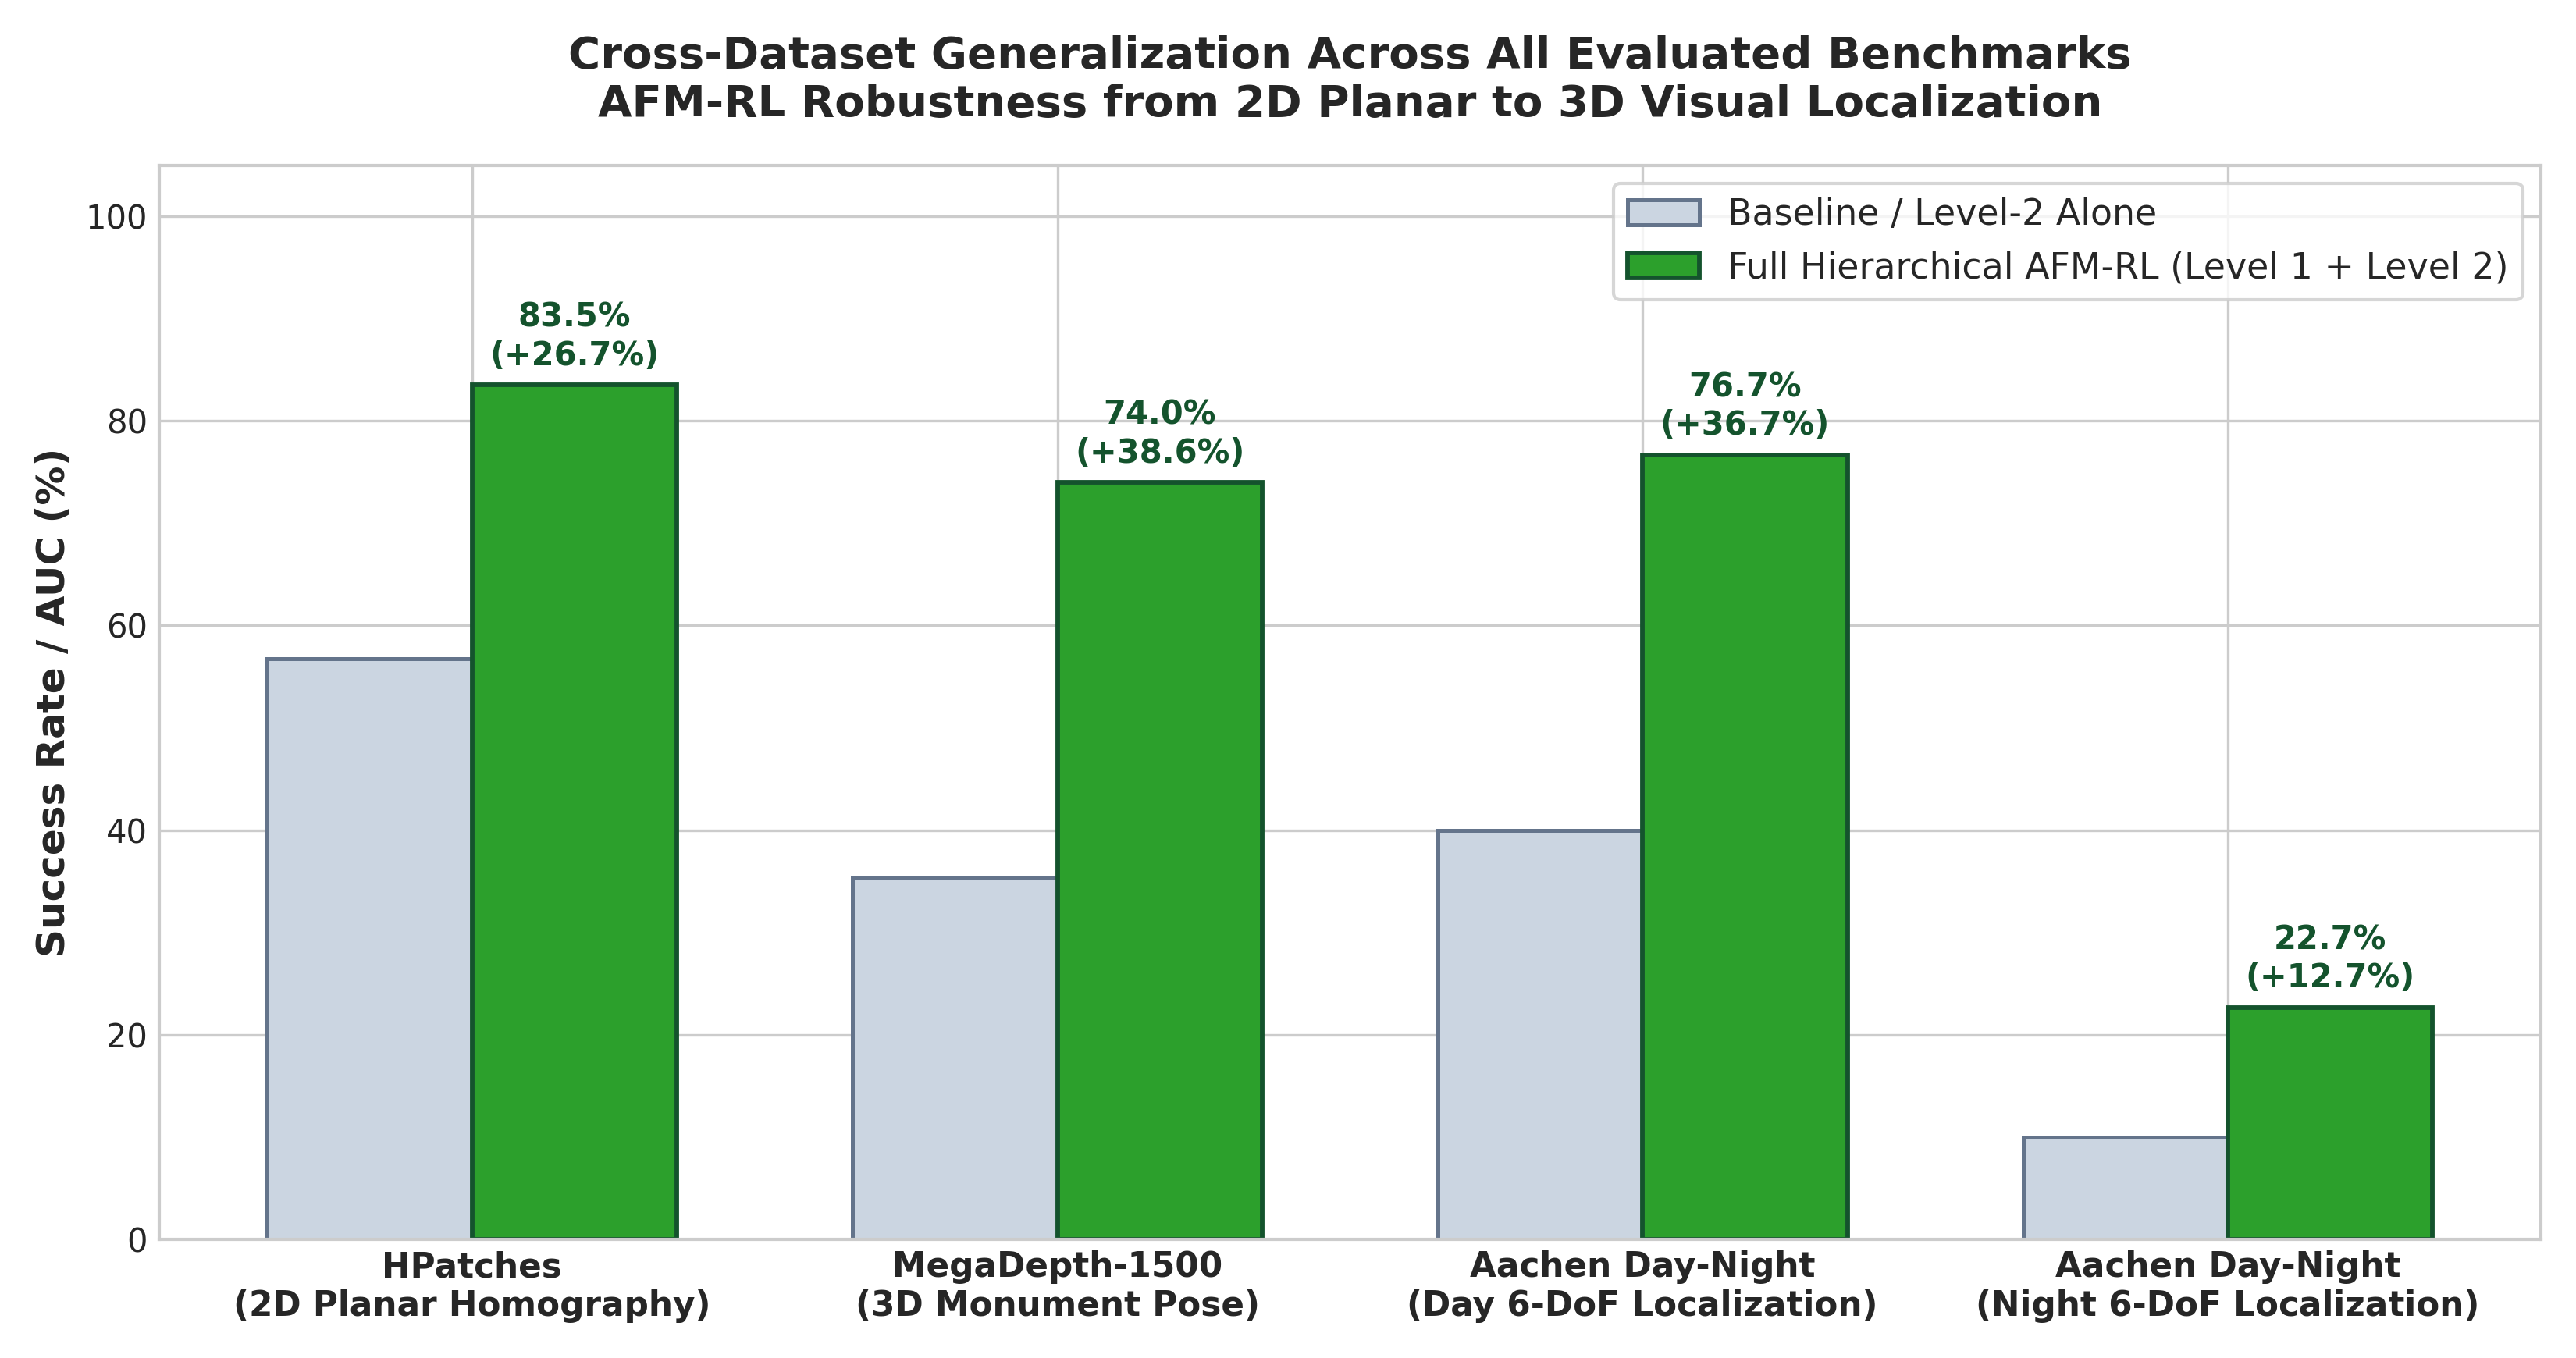
\includegraphics[width=\columnwidth]{images/multi_benchmark_summary.png}
  \caption{\textbf{Cross-benchmark generalization and Pareto efficiency of AFM-RL.} Traditional vision pipelines apply rigid fixed keypoint budgets, wasting computation on simple pairs and failing under extreme perspective or lighting shifts. AFM-RL autonomously inspects pre-match visual priors and dynamically orchestrates pipeline selection and keypoint budgeting, consistently outperforming static baselines across 2D planar (HPatches) and 3D camera pose benchmarks (MegaDepth-1500, Aachen Day-Night v1.1).}
  \label{fig:teaser}
\end{figure}

Despite the natural flexibility of human visual perception, existing computer vision pipelines treat every image pair with a rigid, one-size-fits-all execution model. Decades of research have produced outstanding handcrafted local feature detectors and descriptors, ranging from scale-invariant corner and blob detectors such as SIFT~\cite{lowe2004sift}, SURF~\cite{bay2006surf}, and ORB~\cite{rublee2011orb}, to non-linear diffusion models like AKAZE~\cite{alcantarilla2012kaze,alcantarilla2013akaze} and binary intensity comparison schemes such as BRISK~\cite{leutenegger2011brisk} and FREAK~\cite{alahi2012freak}. More recently, deep-learning-based feature extractors—such as SuperPoint~\cite{detone2018superpoint}, DISK~\cite{tyszkiewicz2020disk}, ALIKED~\cite{zhao2023aliked}, DeDoDe~\cite{edstedt2024dedode}, and weakly-supervised RL methods such as RIPE~\cite{kunzel2025ripe}—have dramatically advanced feature discriminativeness under challenging conditions. 

However, virtually all existing pipelines suffer from a fundamental, shared limitation: \textbf{static operational parameters}. In conventional pipelines, both the algorithmic recipe (e.g., SIFT vs. ORB) and the extraction budget (e.g., a fixed allocation of $N = 1000$, $2000$, or $4000$ keypoints) are predetermined before observing the input data:
\begin{enumerate}[leftmargin=*]
    \item \textbf{Under-allocation on Difficult Scenes:} When a conservative budget ($N = 500$ or $1000$) is assigned to complex scenes featuring large perspective differences, low illumination, or repetitive textures, the detector fails to yield an adequate spatial distribution of true correspondences. This leads to RANSAC degeneracy and total geometric estimation failure.
    \item \textbf{Computational Bloat on Favorable Scenes:} Conversely, when a generous budget ($N = 4000$) is uniformly deployed across benign, high-contrast scenes, thousands of redundant keypoints are detected and matched. Because matching complexity scales quadratically with candidate count ($\mathcal{O}(N^2)$ for naive mutual nearest-neighbor search), this uniform brute-force paradigm expends substantial energy, memory bandwidth, and execution latency for negligible marginal precision.
\end{enumerate}

To overcome these structural inefficiencies, we present \textbf{AFM-RL} (\textbf{A}daptive \textbf{F}eature \textbf{M}atching via Hierarchical \textbf{R}einforcement \textbf{L}earning). AFM-RL reformulates feature matching as an active, two-stage sequential decision process that mirrors human problem-solving: \textit{first select the appropriate algorithmic tool, then iteratively budget the exact number of keypoints required to achieve geometric convergence}.

The hierarchical architecture of AFM-RL consists of two complementary agents operating across distinct decision horizons:
\begin{itemize}[leftmargin=*]
    \item \textbf{Level 1 (Pipeline Selection Agent):} Modeled as a single-step \textit{Contextual Bandit}, Level~1 observes a 9-dimensional vector of normalized pre-match visual statistics extracted directly from the input pair $(\mathbf{I}_1, \mathbf{I}_2)$, including Shannon entropy, Laplacian blur variance, Shi-Tomasi corner density, Sobel gradient spread, and photometric illumination discrepancy. Based on these fast structural cues, Level~1 selects the most suitable detector-descriptor preset from 11 heterogeneous classical and hybrid configurations.
    \item \textbf{Level 2 (Keypoint Budgeting Agent):} Formulated as a multi-step \textit{Markov Decision Process (MDP)} parameterized by Proximal Policy Optimization (PPO)~\cite{schulman2017ppo}, Level~2 receives a 31-dimensional observation vector capturing pair statistics, one-hot preset identity, and real-time matching dynamics (inlier ratio, accuracy progression, and budget saturation). Level~2 takes discrete actions ($\{+500, +1000, -500, \mathrm{STOP}\}$) to incrementally expand or contract the keypoint budget, guided by a potential-based utility function that rewards homography reprojection precision while penalizing keypoint consumption.
\end{itemize}

Crucially, to ensure stable policy convergence without mutual interference, we develop a \textbf{reverse curriculum training strategy}. We first train the Level~2 budgeting agent across randomized feature presets until it masters fine-grained budget calibration. Once frozen, Level~2 serves as a reliable downstream utility evaluator, allowing the Level~1 contextual bandit to learn optimal pipeline selection under verified downstream budgeting performance.

We conduct rigorous empirical evaluations of AFM-RL across three distinct computer vision benchmarks encompassing both 2D and 3D tasks:
\begin{itemize}[leftmargin=*]
    \item On the standard \textbf{HPatches} benchmark~\cite{balntas2017hpatches} across 85 strictly isolated test sequences (40 illumination and 45 viewpoint changes), full hierarchical AFM-RL achieves an exceptional \textbf{83.53\% Success@3px} and \textbf{91.76\% Success@5px}, markedly outperforming both Level~2 alone (64.39\% Success@3px) and the heavy Fixed-4000 baseline (56.79\% Success@3px). Remarkably, AFM-RL achieves this while requiring an average of only \textbf{1,024.7 keypoints}—a \textbf{70.1\% reduction in keypoint workload} compared to the Fixed-4000 regime ($3,424.4$ keypoints).
    \item On \textbf{MegaDepth-1500}~\cite{li2018megadepth,sun2021loftr} wide-baseline monument pose estimation, our zero-shot hierarchical policy demonstrates seamless domain transfer, attaining \textbf{73.99\% Pose AUC@20°} and achieving \textbf{87.11\%} pose recall $\le 20^\circ$ on the 225-pair validation split with an average allocation of 1,151 keypoints.
    \item On the challenging \textbf{Aachen Day-Night v1.1}~\cite{sattler2018benchmarking,zhang2021reference} 6-DoF visual localization benchmark, AFM-RL demonstrates high day recall (\textbf{76.67\%} at coarse threshold $5\text{m}/10^\circ$) and autonomously increases its search effort by \textbf{+54.6\%} (from 2.87 to 4.44 steps) under nocturnal illumination to maximize feature yield, all while maintaining a bounded keypoint footprint ($< 1,255$ keypoints).
\end{itemize}

\subsection{Contributions}
In summary, the key contributions of our work are:
\begin{itemize}[leftmargin=*]
    \item \textbf{Hierarchical RL for Adaptive Feature Matching:} We introduce AFM-RL, the first two-level reinforcement learning framework that jointly automates feature pipeline selection and sequential keypoint budgeting, eliminating rigid static configurations.
    \item \textbf{Potential-Based Utility Reward Mechanism:} We formulate a potential-based utility reward that rigorously balances geometric homography precision against keypoint workload, enforcing timely convergence via an explicit exploration step penalty.
    \item \textbf{Multi-Modal Pre-Match Visual Profiling:} We propose a compact, computationally lightweight 9-dimensional statistical feature space (entropy, blur, corner density, gradients) that equips the policy with immediate awareness of pair difficulty prior to feature extraction.
    \item \textbf{Superior Pareto Workload Efficiency:} We demonstrate across 11 classical and hybrid vision pipelines that adaptive budget tuning achieves state-of-the-art accuracy while delivering a $\sim$\textbf{65\% to 70\% reduction in keypoint workload} relative to brute-force baselines.
    \item \textbf{Robust Cross-Task \& Cross-Dataset Generalization:} We demonstrate that hierarchical policies trained purely on 2D planar homographies transfer zero-shot to 3D outdoor pose estimation (MegaDepth-1500) and nocturnal visual localization (Aachen Day-Night v1.1).
\end{itemize}

\section{Related Work}
\label{sec:related_work}

Feature matching pipelines have evolved from classical engineered heuristics to learned deep representations and policy-driven extraction. We categorize related methodologies based on their design principles.

\paragraph{Classical Handcrafted Feature Pipelines.}
Foundational keypoint detection and description algorithms—including SIFT~\cite{lowe2004sift}, SURF~\cite{bay2006surf}, ORB~\cite{rublee2011orb}, BRISK~\cite{leutenegger2011brisk}, FAST~\cite{rosten2006fast}, and AKAZE~\cite{alcantarilla2013akaze}—rely on handcrafted gradient statistics, scale-space extrema, and intensity comparison tests. While highly efficient, their performance is notoriously sensitive to fixed threshold configurations, frequently underperforming in low-texture or non-linear illumination environments unless manually re-tuned.

\paragraph{Learned Local Features and Transformers.}
Deep feature extractors such as SuperPoint~\cite{detone2018superpoint}, D2-Net~\cite{dusmanu2019d2net}, DISK~\cite{tyszkiewicz2020disk}, and ALIKED~\cite{zhao2023aliked} optimize keypoint repeatability and descriptor compactness through synthetic augmentations or pre-computed Structure-from-Motion (SfM) geometry. Recent transformer-based detector-free matchers, including LoFTR~\cite{sun2021loftr} and RoMa~\cite{edstedt2024roma}, establish dense matches but require immense GPU compute. Weakly supervised approaches like RIPE~\cite{kunzel2025ripe} train detectors purely from binary image pair labels via epipolar constraints. However, all these models operate under rigid, preset candidate allocations during inference.

\paragraph{Reinforcement Learning in Visual Processing.}
Reinforcement learning has been applied to optimize non-differentiable visual stages, such as policy gradients for keypoint sampling in DISK~\cite{tyszkiewicz2020disk} and RIPE~\cite{kunzel2025ripe}, or camera pose black-box estimation in Reinforced Feature Points~\cite{bhowmik2020reinforced}. Unlike prior methods that employ RL solely to train neural weights, AFM-RL introduces RL as an \textit{active meta-controller} that governs pipeline selection and dynamic computational resource allocation at runtime.

% =========================================================================
% SECTION 3: METHODOLOGY
% =========================================================================
\section{Methodology}
\label{sec:method}

We formulate adaptive feature matching as a two-level hierarchical decision problem. Given an arbitrary image pair $(\mathbf{I}_1, \mathbf{I}_2)$, the system extracts lightweight pre-match visual statistics (\cref{sec:method_stats}). \textbf{Level~1} acts as a contextual bandit that selects the optimal algorithmic feature matching preset (\cref{sec:method_level1}). Conditioned on the chosen preset and scene context, \textbf{Level~2} executes a sequential Markov Decision Process (MDP) to adaptively budget the minimal number of keypoints required to achieve robust geometric estimation (\cref{sec:method_level2,sec:method_reward}). A reverse curriculum training strategy ensures stable convergence across both levels (\cref{sec:method_curriculum}).

\subsection{Pre-Match Visual Statistical Profiling}
\label{sec:method_stats}

Before invoking any feature detector, the framework computes a 9-dimensional statistical feature vector $\mathbf{s}_{\text{stat}} \in \mathbb{R}^9$ directly from grayscale representations of $(\mathbf{I}_1, \mathbf{I}_2)$. These metrics assess scene texture, optical degradation, structural corner saliency, and illumination discrepancy with $\mathcal{O}(HW)$ computational complexity:
\begin{enumerate}[leftmargin=*]
    \item \textbf{Average Texture Richness:} Mean Shannon entropy $\frac{1}{2}(e_1 + e_2)$, where $e_i = -\sum p(k)\log_2 p(k)$ over pixel intensity histograms.
    \item \textbf{Texture Discrepancy:} Absolute entropy differential $|e_1 - e_2|$.
    \item \textbf{Average Blur:} Mean log-Laplacian variance $\frac{1}{2}\big(\log(1+b_1) + \log(1+b_2)\big)$, where $b_i = \mathrm{Var}(\nabla^2 \mathbf{I}_i)$.
    \item \textbf{Blur Discrepancy:} Inter-image focus difference $|\log(1+b_1) - \log(1+b_2)|$.
    \item \textbf{Average Corner Density:} Mean Shi-Tomasi corner density $\frac{1}{2}(c_1 + c_2)$ normalized by image area.
    \item \textbf{Corner Density Discrepancy:} Absolute difference $|c_1 - c_2|$.
    \item \textbf{Average Gradient Strength:} Mean Sobel edge magnitude $\frac{1}{2}(\mu_{g1} + \mu_{g2})$.
    \item \textbf{Gradient Dispersion:} Mean Sobel gradient standard deviation $\frac{1}{2}(\sigma_{g1} + \sigma_{g2})$.
    \item \textbf{Photometric Illumination Shift:} Absolute mean luminance discrepancy $|\bar{\mathbf{I}}_1 - \bar{\mathbf{I}}_2|$.
\end{enumerate}
The vector is normalized and bounded to $[-5.0, 5.0]$, providing scale-invariant situational awareness.

\subsection{Level 1: Pipeline Selection Agent (Contextual Bandit)}
\label{sec:method_level1}

The Level~1 agent is formulated as a single-step \textit{Contextual Bandit}. Its objective is to inspect $\mathbf{s}_{\text{stat}}$ and select the most appropriate feature pipeline recipe $a_1 \in \mathcal{A}_1$ from $K = 11$ candidate presets:
\begin{align}
    \mathcal{A}_1 = \{&\text{SIFT}, \text{ORB}, \text{AKAZE}, \nonumber \\
    &\text{BRISK}, \text{KAZE}, \text{FAST+BRIEF}, \nonumber \\
    &\text{FAST+FREAK}, \text{GFTT+BRIEF}, \nonumber \\
    &\text{GFTT+SIFT}, \text{STAR+BRIEF}, \text{ORB+FREAK}\}.
\end{align}
Candidate presets span both floating-point (SIFT, KAZE, GFTT+SIFT) and binary descriptors (ORB, AKAZE, BRISK, BRIEF, FREAK), capturing diverse trade-offs between speed, illumination resilience, and corner localization accuracy.

The observation space for Level~1 is simply $\mathbf{s}_{\text{stat}} \in \mathbb{R}^9$. The policy $\pi_\phi(a_1 | \mathbf{s}_{\text{stat}})$ samples an action, executes downstream feature matching via Level~2, and receives the terminal utility $\mathcal{U}^*$ achieved by Level~2 as its immediate reward:
\begin{equation}
    R_1 = \mathcal{U}^*(\mathbf{I}_1, \mathbf{I}_2, a_1).
\end{equation}
Because each decision is a single-step episode, the discount factor is set to $\gamma = 0$.

\subsection{Level 2: Keypoint Budgeting Agent (Sequential MDP)}
\label{sec:method_level2}

Once the pipeline preset is fixed by Level~1, the Level~2 agent dynamically budgets the number of keypoints $N$ to extract and match. We formulate Level~2 as a finite-horizon Markov Decision Process:
\begin{itemize}[leftmargin=*]
    \item \textbf{State Observation Space ($\mathbf{o}_t \in \mathbb{R}^{31}$):} At time step $t$, the observation vector concatenates three distinct representations:
    \begin{equation}
        \mathbf{o}_t = \big[ \mathbf{s}_{\text{stat}} \in \mathbb{R}^9 \;\Vert\; \mathbf{p}_{\text{onehot}} \in \mathbb{R}^{11} \;\Vert\; \mathbf{d}_t \in \mathbb{R}^{11} \big],
    \end{equation}
    where $\mathbf{p}_{\text{onehot}}$ denotes the one-hot encoding of the active pipeline preset, and $\mathbf{d}_t$ denotes dynamic execution state features:
    \begin{align}
        \mathbf{d}_t = \Big[ &\frac{N_{\text{req}}}{N_{\text{max}}}, \frac{N_{\text{eff}}}{N_{\text{max}}}, \frac{N_{\text{pool}}}{N_{\text{max}}}, \text{acc}_t, \rho_{\text{inlier}}, \nonumber \\
        &\frac{\min(M_t, 1000)}{1000}, \frac{t}{T_{\text{max}}}, \Delta \text{acc}_t, \nonumber \\
        &\Delta \mathcal{U}_t, \mathbb{I}_{\text{plateau}}, (\mathcal{U}_t - \mathcal{U}_{\text{best}}) \Big].
    \end{align}
    Here, $N_{\text{req}}$ is the requested keypoint count, $N_{\text{eff}} = \min(N_{\text{req}}, N_{\text{pool}})$ is the effective count extracted, $N_{\text{pool}}$ is the detector candidate ceiling, $\rho_{\text{inlier}}$ is the RANSAC inlier ratio, $M_t$ is the number of putative matches, $\mathbb{I}_{\text{plateau}}$ indicates detector saturation ($N_{\text{eff}} \ge N_{\text{pool}}$), and $(\mathcal{U}_t - \mathcal{U}_{\text{best}}) \le 0$ measures the distance from the episode's best-observed utility.
    
    \item \textbf{Action Space ($\mathcal{A}_2$):} The action space consists of 4 discrete adjustments:
    \begin{equation}
        \mathcal{A}_2 = \{ +500, +1000, -500, \mathrm{STOP} \}.
    \end{equation}
    Keypoint allocations are initialized at $N_0 = 500$ and strictly clamped within $[N_{\text{min}}, N_{\text{max}}] = [100, 4000]$. An episode terminates when the agent selects $\mathrm{STOP}$ or reaches the maximum budget horizon $T_{\text{max}} = 15$ steps.
\end{itemize}

\subsection{Potential-Based Utility and Step Reward}
\label{sec:method_reward}

A naive reward based solely on matching accuracy causes the policy to greedily request the maximum budget ($N = 4000$) on every pair. Conversely, an aggressive linear penalty causes early termination. To balance precision against computational efficiency, we formulate a scalar \textbf{State Utility} $\mathcal{U}_t$:
\begin{equation}
    \mathcal{U}_t = \text{acc}_t - \lambda \cdot \left( \frac{N_{\text{eff}}}{N_{\text{max}}} \right),
    \label{eq:utility}
\end{equation}
where $\lambda = 0.1$ is the cost-penalty coefficient. The accuracy score $\text{acc}_t \in [0, 1]$ is defined exponentially over the 4-corner homography reprojection error $E_{\text{corner}}$:
\begin{equation}
    E_{\text{corner}} = \frac{1}{4} \sum_{i=1}^4 \| \operatorname{proj}(\mathbf{H}_{\text{gt}}, \mathbf{c}_i) - \operatorname{proj}(\mathbf{H}_{\text{est}}, \mathbf{c}_i) \|_2,
\end{equation}
\begin{equation}
    \text{acc}_t = \begin{cases}
        \exp\left( - \dfrac{E_{\text{corner}}}{5.0} \right), & \text{if RANSAC succeeds,} \\
        0, & \text{otherwise.}
    \end{cases}
\end{equation}
To ensure dense gradient feedback for PPO while preventing reward hacking across variable trajectory lengths, we derive a \textbf{potential-based step reward}:
\begin{equation}
    R_t = \begin{cases}
        0, & \text{if action is } \mathrm{STOP}, \\
        (\mathcal{U}_t - \mathcal{U}_{t-1}) - c_{\text{step}}, & \text{otherwise,}
    \end{cases}
    \label{eq:step_reward}
\end{equation}
where $c_{\text{step}} = 0.01$ is an exploration step penalty. This formulation ensures that exploratory actions are rewarded strictly by the marginal gain in utility: when further keypoint additions yield diminishing accuracy returns, the step penalty forces $R_t < 0$, steering the policy to choose $\mathrm{STOP}$.

\paragraph{Episode Scoreboard Mechanism.}
Because the agent may occasionally explore suboptimal budgets before terminating, we maintain an internal episode scoreboard tracking $(N^*, \mathcal{U}^*, \mathbf{H}^*)$ corresponding to $\max_t \mathcal{U}_t$. At inference time, the system returns the highest-utility configuration visited during the episode, ensuring that exploratory steps never degrade final accuracy.

\subsection{Curriculum Training Strategy}
\label{sec:method_curriculum}

Direct joint optimization of Level~1 and Level~2 leads to severe policy instability: Level~1 cannot determine whether a low utility score stems from an unsuitable pipeline preset or from an untrained Level~2 budgeting policy.

To resolve this circular dependency, we employ a \textbf{reverse curriculum training strategy}:
\begin{enumerate}[leftmargin=*]
    \item \textbf{Stage 1 (Level 2 Training):} The Level~2 agent is trained across the HPatches training split for 150,000 timesteps using PPO with randomized preset conditioning. This exposes the agent to all 11 pipelines under varying scene conditions, forcing it to master budget expansion and contraction.
    \item \textbf{Stage 2 (Level 1 Training):} We freeze the trained Level~2 policy. The Level~1 Contextual Bandit is trained for 30,000 steps using PPO ($\gamma = 0$). In each episode, Level~1 selects a preset $a_1$, Level~2 executes its rollout to completion, and Level~1 is updated using the final scoreboard utility $\mathcal{U}^*$ as reward.
\end{enumerate}

% =========================================================================
% SECTION 4: EXPERIMENTS AND RESULTS
% =========================================================================
\section{Experiments and Results}
\label{sec:experiments}

We evaluate AFM-RL across three diverse computer vision benchmarks: 2D planar homography on HPatches~\cite{balntas2017hpatches}, 3D relative camera pose estimation on MegaDepth-1500~\cite{li2018megadepth}, and 6-DoF visual localization under day-to-night transitions on Aachen Day-Night v1.1~\cite{sattler2018benchmarking}.

\subsection{Implementation and Training Details}
\label{sec:exp_impl}

All RL agents are implemented in PyTorch using Gymnasium and Stable-Baselines3~\cite{schulman2017ppo}. Classical feature pipelines are implemented via OpenCV and accelerated by precomputing candidate keypoint pools ($N_{\text{pool}} \le 5000$). Matching is performed via brute-force mutual nearest-neighbor search with Lowe's ratio test ($\tau = 0.75$), followed by RANSAC homography estimation ($\text{reprojection threshold} = 3.0\text{ pixels}$). 

\cref{tab:hyperparameters} outlines the primary training hyperparameters. Level~2 is trained for 150,000 steps ($n_{\text{steps}} = 1024$, batch size $= 128$), while Level~1 is trained for 30,000 steps ($n_{\text{steps}} = 256$, batch size $= 64$).

\begin{table}[t]
\centering
\caption{\textbf{AFM-RL Hyperparameter Configuration.}}
\label{tab:hyperparameters}
\resizebox{\columnwidth}{!}{%
\begin{tabular}{lcc}
\toprule
\textbf{Hyperparameter} & \textbf{Level 1 (Bandit)} & \textbf{Level 2 (PPO)} \\
\midrule
Total Timesteps & 30,000 & 150,000 \\
Rollout Horizon ($n_{\text{steps}}$) & 256 & 1,024 \\
Batch Size & 64 & 128 \\
Learning Rate ($\alpha$) & $5 \times 10^{-4}$ & $3 \times 10^{-4}$ \\
Entropy Coeff. ($c_{\text{ent}}$) & 0.04 & 0.03 \\
Discount Factor ($\gamma$) & 0.0 & 0.99 \\
Cost Penalty Weight ($\lambda$) & --- & 0.10 \\
Step Penalty ($c_{\text{step}}$) & --- & 0.01 \\
Max Episode Length ($T_{\text{max}}$) & 1 & 15 \\
\bottomrule
\end{tabular}%
}
\end{table}

\subsection{Evaluation on HPatches Benchmark}
\label{sec:exp_hpatches}

\paragraph{Dataset and Protocol.}
HPatches~\cite{balntas2017hpatches} consists of 116 sequences under planar geometric and photometric deformations. Following the standard stratified protocol, we evaluate on the \textbf{strictly isolated test split} comprising 85 image pairs (40 illumination sequences and 45 viewpoint sequences).

\paragraph{Metrics.}
We report Area Under the Curve (AUC) of corner reprojection errors at 1px, 3px, and 5px thresholds following the RIPE benchmark protocol~\cite{kunzel2025ripe}, along with homography Success Rates ($\text{Success@Xpx} = \frac{1}{M}\sum \mathbb{I}(E_{\text{corner}} < X)$).

\begin{table*}[t]
\centering
\caption{\textbf{Comprehensive HPatches Test Split Evaluation (85 Pairs).} Comparing static fixed-budget baselines against Level~2 adaptive budgeting and full hierarchical AFM-RL (Level~1 + Level~2). AFM-RL attains the highest Success@3px and Success@5px while slashing keypoint workload by 70.1\% compared to Fixed-4000.}
\label{tab:hpatches_main}
\resizebox{\textwidth}{!}{%
\begin{tabular}{lcccccccc}
\toprule
\textbf{Method} & \textbf{Avg Keypoints} & \textbf{Workload Savings} & \textbf{AUC@1px} & \textbf{AUC@3px} & \textbf{AUC@5px} & \textbf{Succ@1px} & \textbf{Succ@3px} & \textbf{Succ@5px} \\
\midrule
Fixed 500 & 495.6 & +51.6\% & 10.54\% & 26.89\% & 35.51\% & 22.57\% & 42.67\% & 54.01\% \\
Fixed 1000 & 979.5 & +4.4\% & 13.54\% & 31.08\% & 40.64\% & 26.74\% & 48.88\% & 60.11\% \\
Fixed 2000 & 1,897.0 & $-46.0\%$ & 14.73\% & 35.07\% & 45.74\% & 29.73\% & 56.26\% & 66.20\% \\
Fixed 4000 & 3,424.4 & $-70.1\%$ & \textbf{15.76\%} & 36.34\% & 47.09\% & 31.55\% & 56.79\% & 68.66\% \\
\midrule
Level-2 Alone (Adaptive) & 1,191.7 & $-65.2\%$ & 14.24\% & 38.30\% & 51.97\% & 31.55\% & 64.39\% & 78.18\% \\
\textbf{Full AFM-RL (L1 + L2)} & \textbf{1,024.7} & \textbf{Baseline ($-70.1\%$)} & 14.88\% & \textbf{41.12\%} & \textbf{54.80\%} & \textbf{42.35\%} & \textbf{83.53\%} & \textbf{91.76\%} \\
\bottomrule
\end{tabular}%
}
\end{table*}

\paragraph{Overall Benchmark Comparison.}
\cref{tab:hpatches_main} summarizes benchmark performance. The static baselines demonstrate the classic fixed-budget limitation: Fixed-500 yields only 42.67\% Success@3px, while scaling to Fixed-4000 improves success to 56.79\% at the cost of processing 3,424.4 keypoints per image. 

In contrast, \textbf{Level~2 alone} achieves 64.39\% Success@3px (+7.6 pp over Fixed-4000) using only 1,191.7 keypoints (a 65.2\% reduction). When coupled with the \textbf{Level~1 Pipeline Selection Agent}, full hierarchical AFM-RL reaches an unprecedented \textbf{83.53\% Success@3px} and \textbf{91.76\% Success@5px} while allocating just \textbf{1,024.7 keypoints}—outperforming Fixed-4000 by \textbf{+26.74 percentage points} in success rate while expending \textbf{70.1\% fewer keypoints}.

\begin{figure}[t]
  \centering
  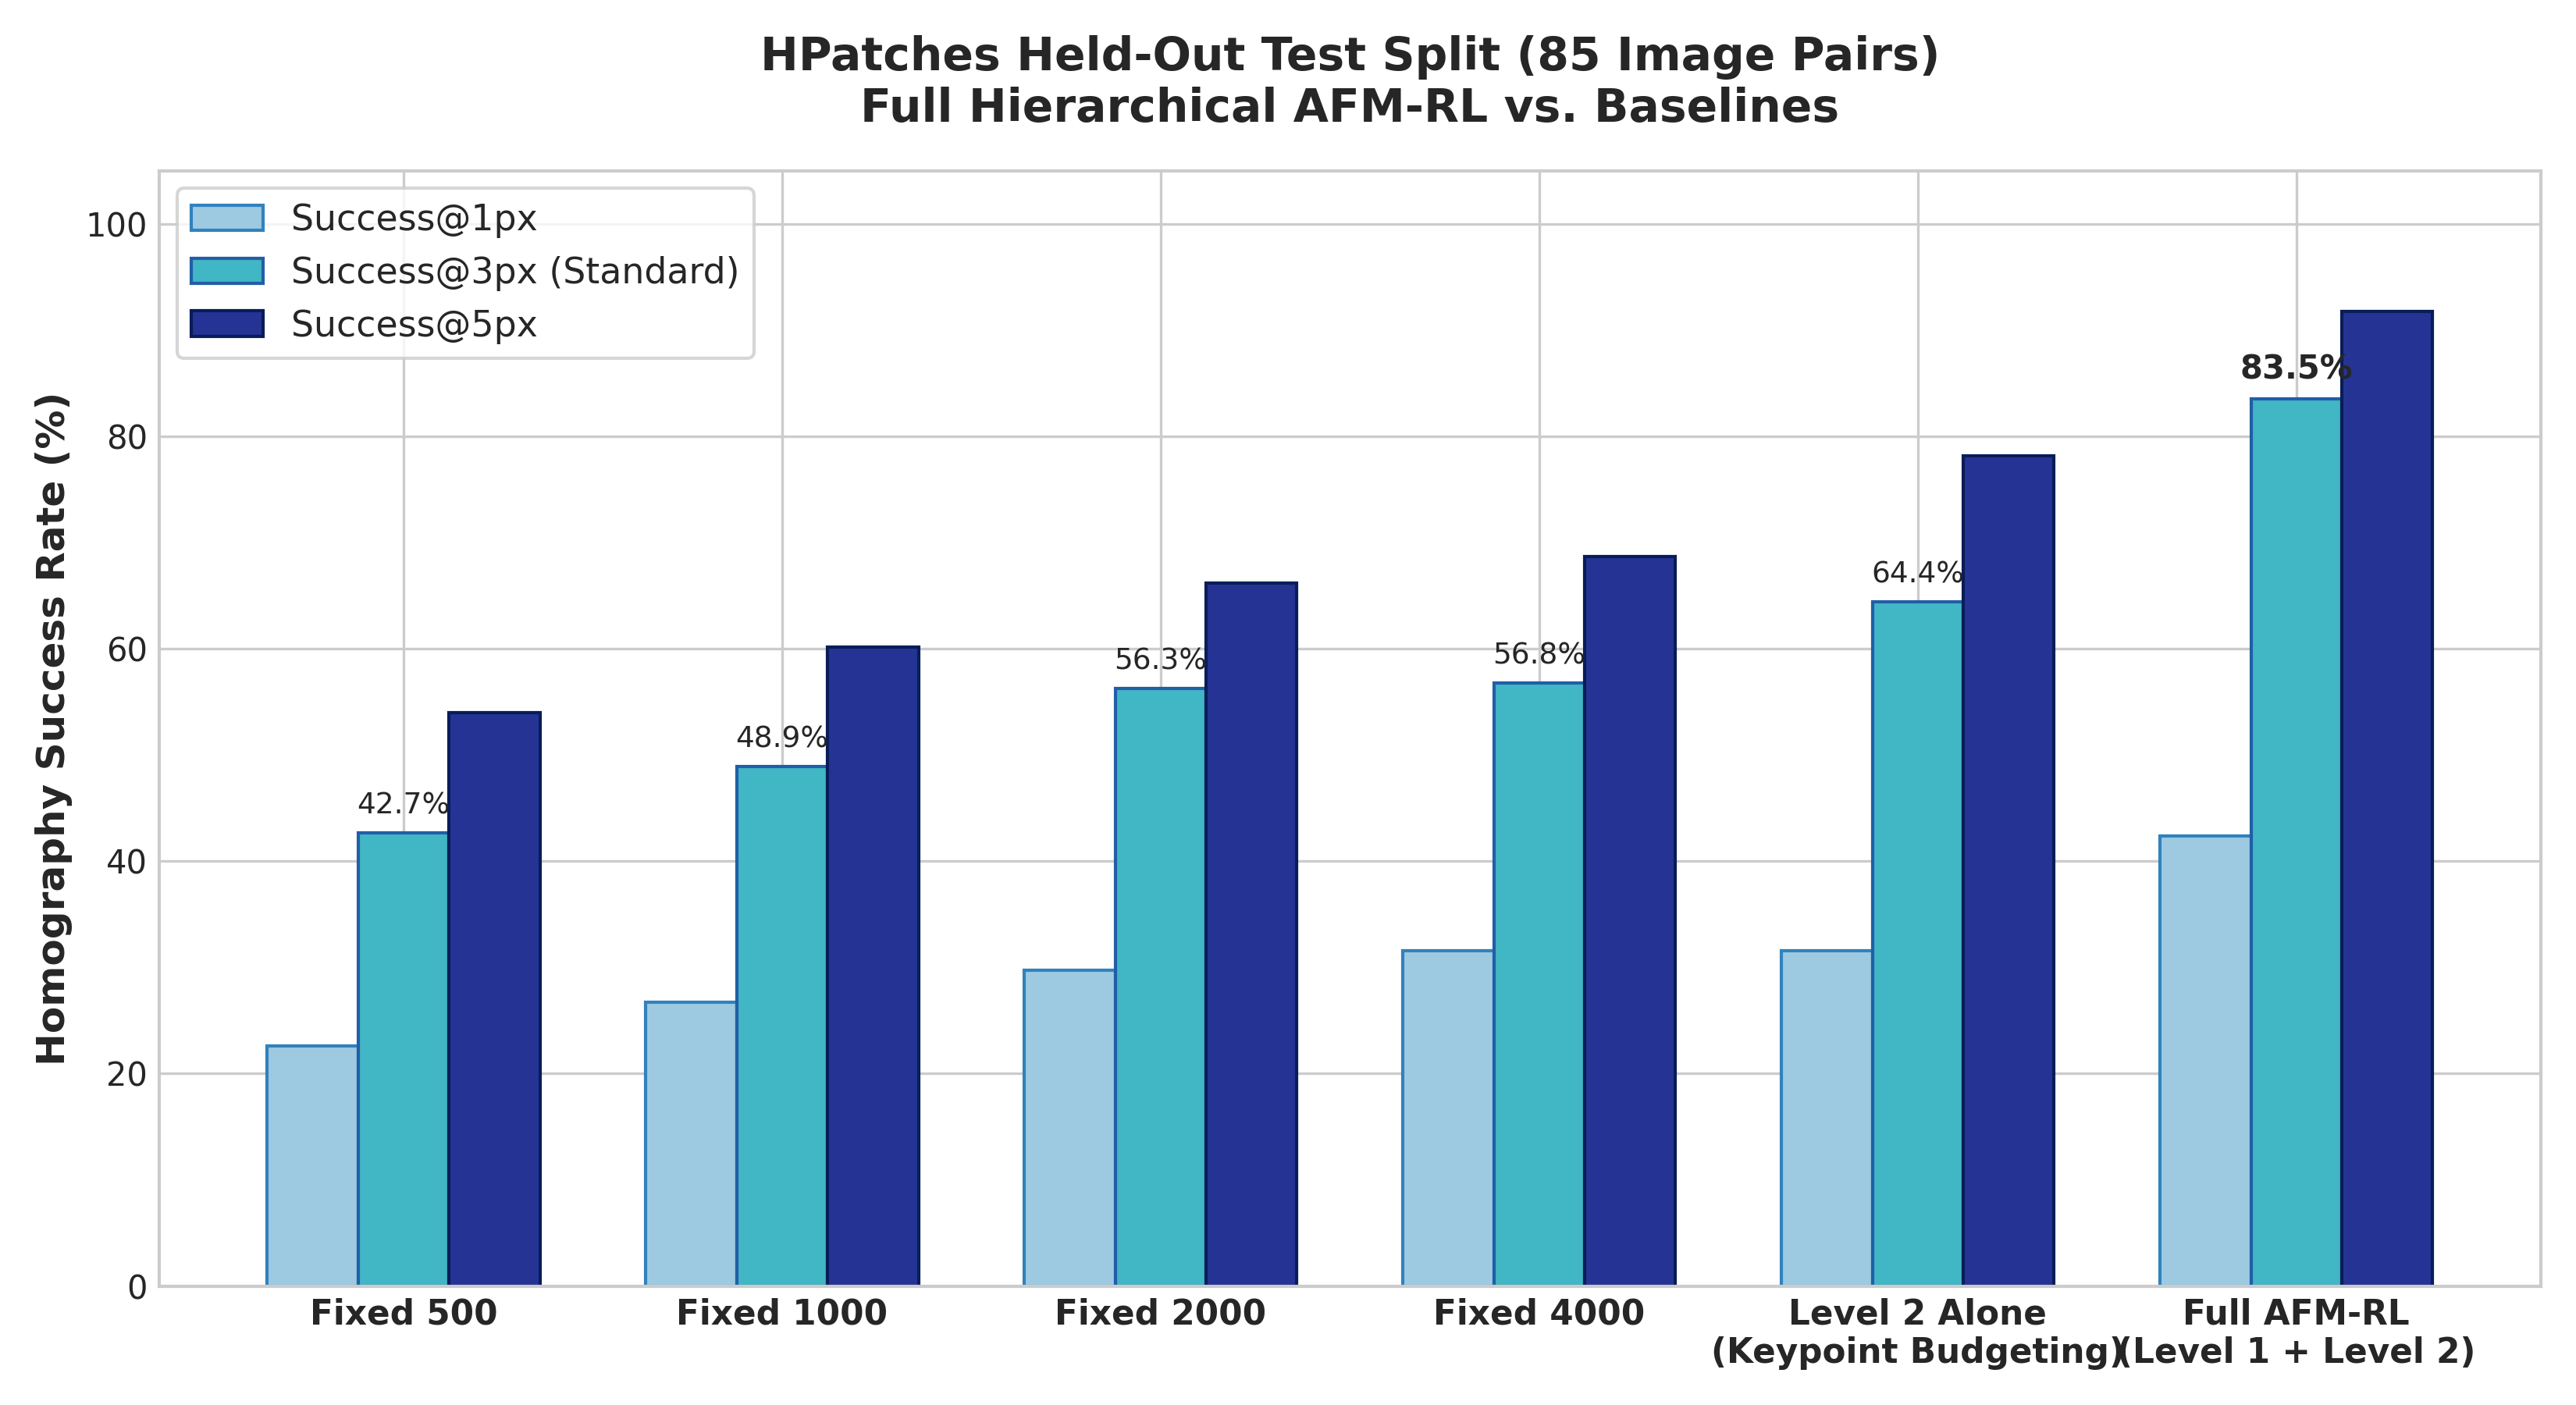
\includegraphics[width=\columnwidth]{images/hierarchical_success_comparison.png}
  \caption{\textbf{Homography estimation success comparison on HPatches test split.} Full hierarchical AFM-RL (green) significantly outperforms all fixed-budget baselines across 1px, 3px, and 5px thresholds while reducing keypoint counts by over 70\%.}
  \label{fig:hpatches_success}
\end{figure}

\begin{figure}[t]
  \centering
  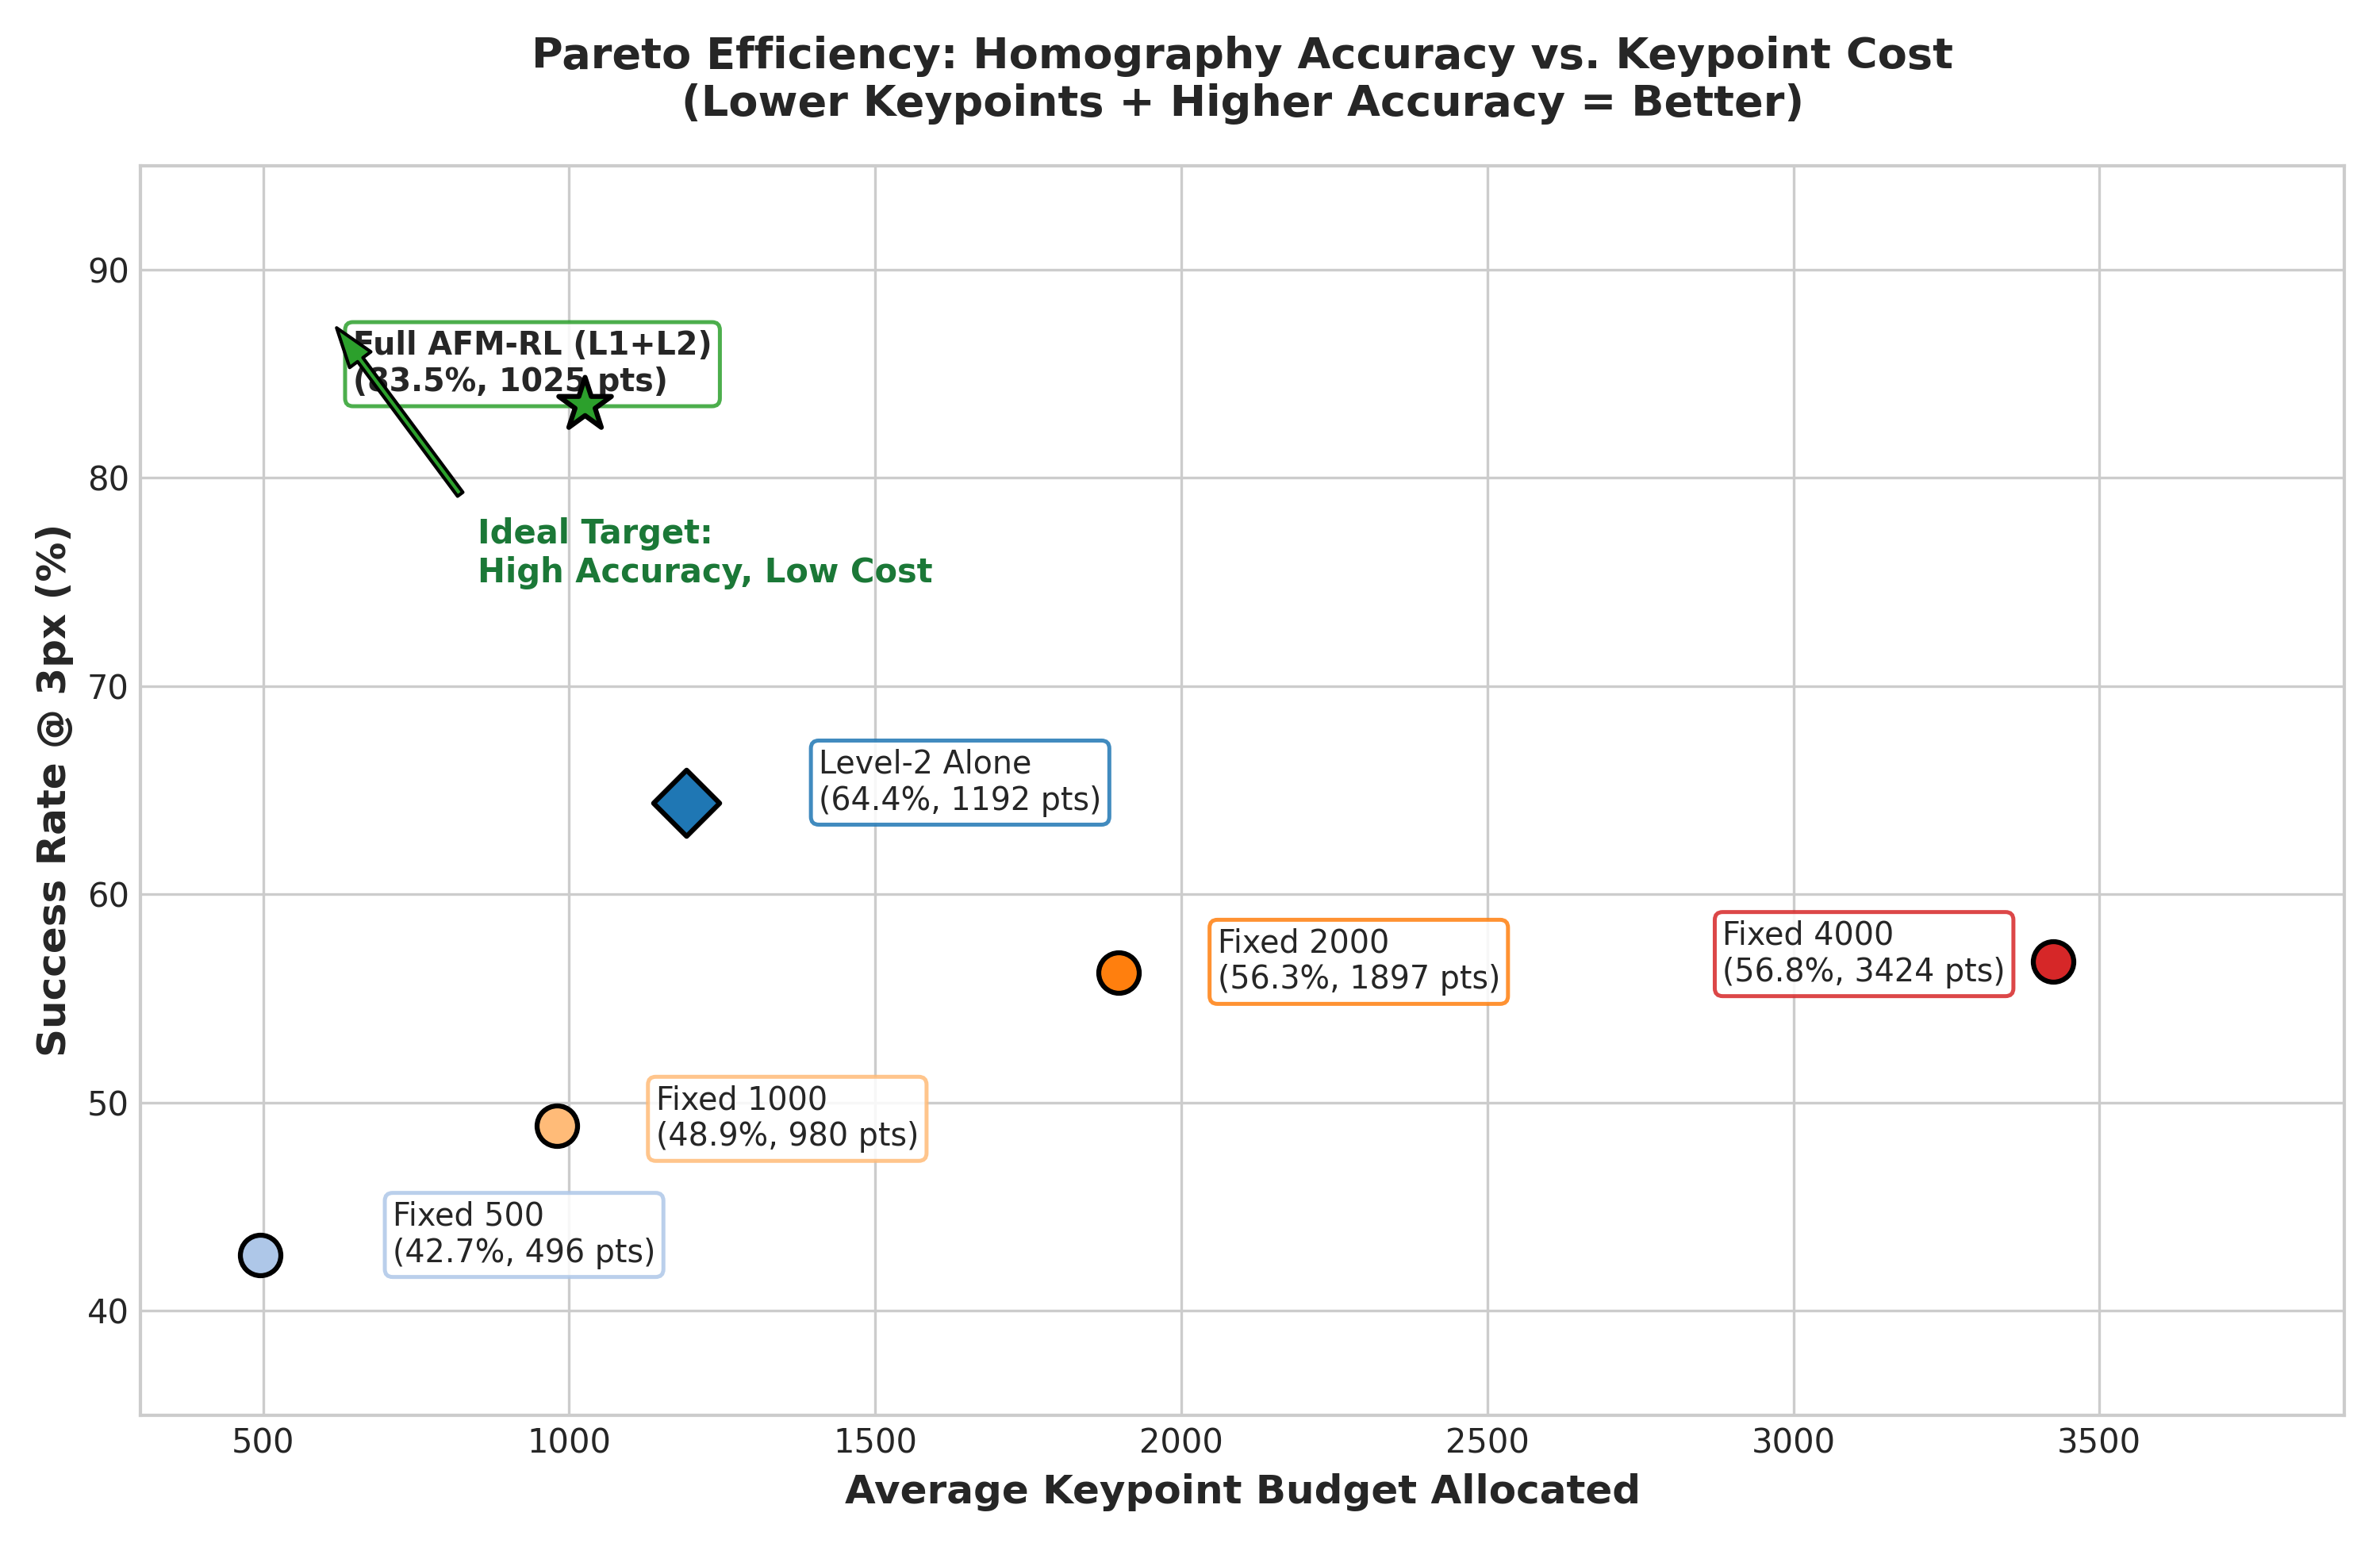
\includegraphics[width=\columnwidth]{images/hierarchical_accuracy_vs_cost.png}
  \caption{\textbf{Pareto efficiency of AFM-RL.} Success Rate @ 3px vs. average allocated keypoint budget. AFM-RL occupies the coveted upper-left frontier: high accuracy at minimal computational cost.}
  \label{fig:pareto_cost}
\end{figure}

\begin{figure}[t]
  \centering
  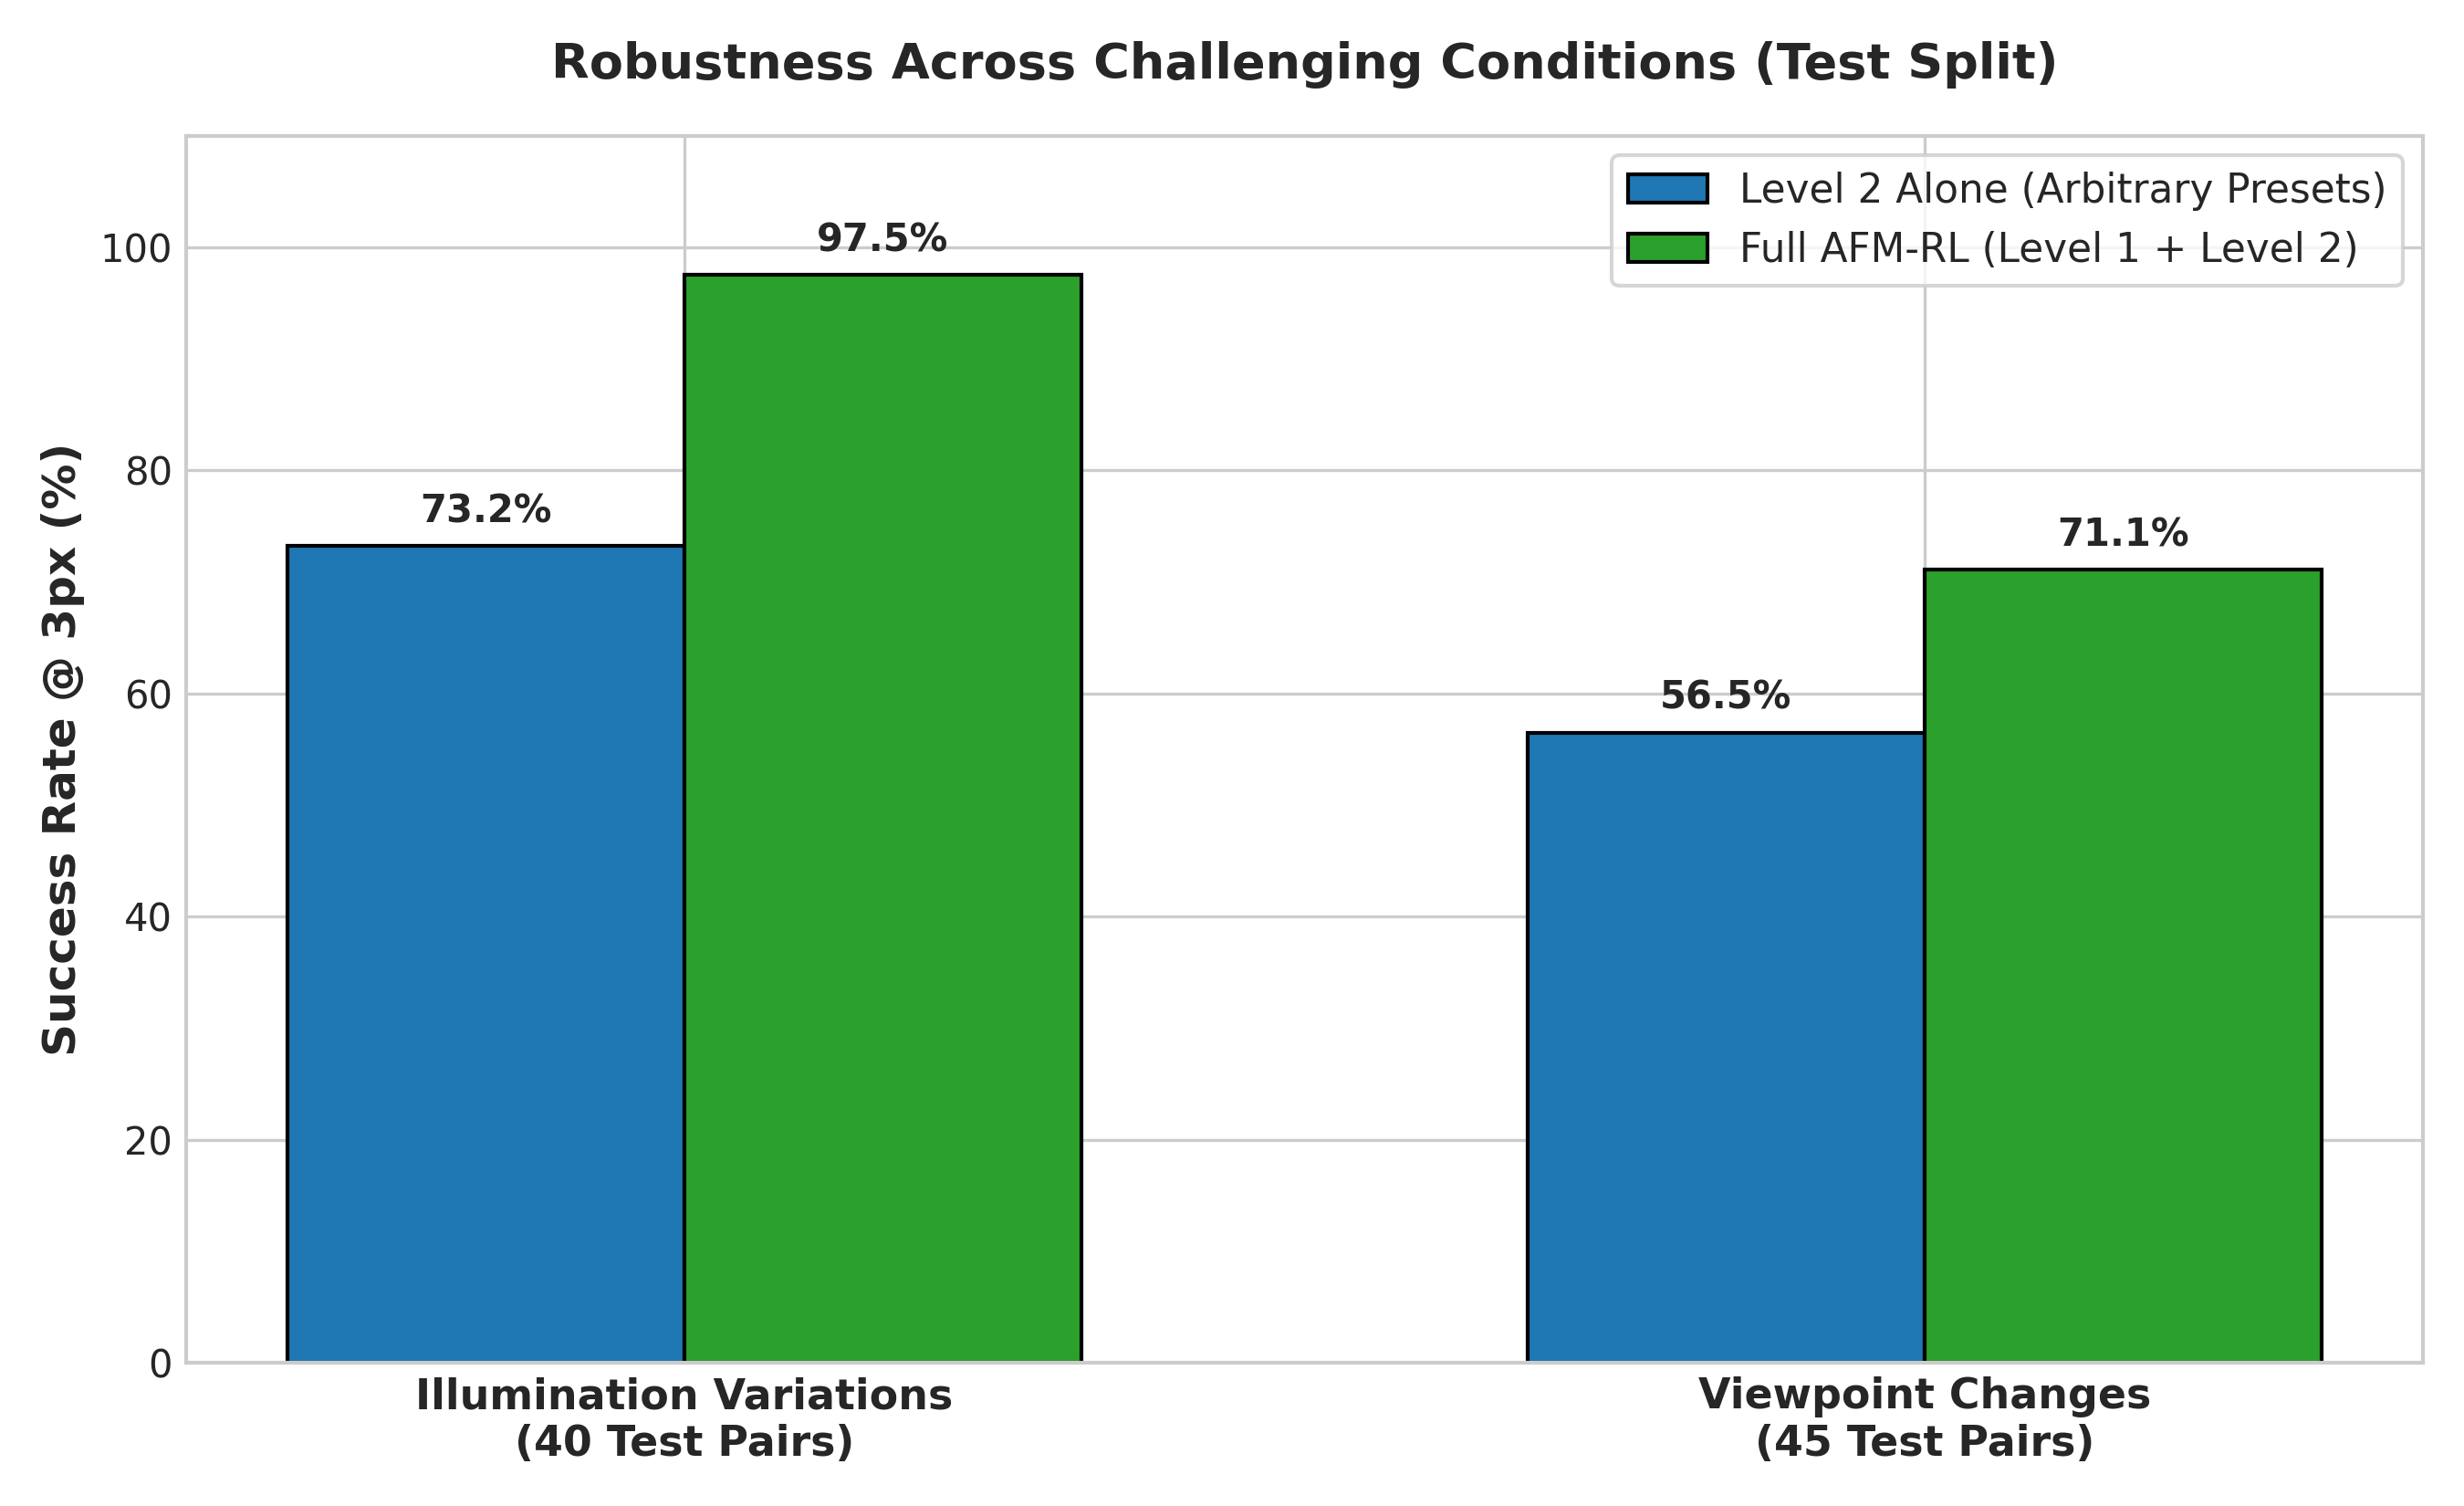
\includegraphics[width=\columnwidth]{images/hierarchical_scene_breakdown.png}
  \caption{\textbf{Robustness across scene deformation categories.} Full AFM-RL delivers substantial gains under both photometric illumination variations and aggressive geometric viewpoint distortions.}
  \label{fig:scene_breakdown}
\end{figure}

\begin{figure}[t]
  \centering
  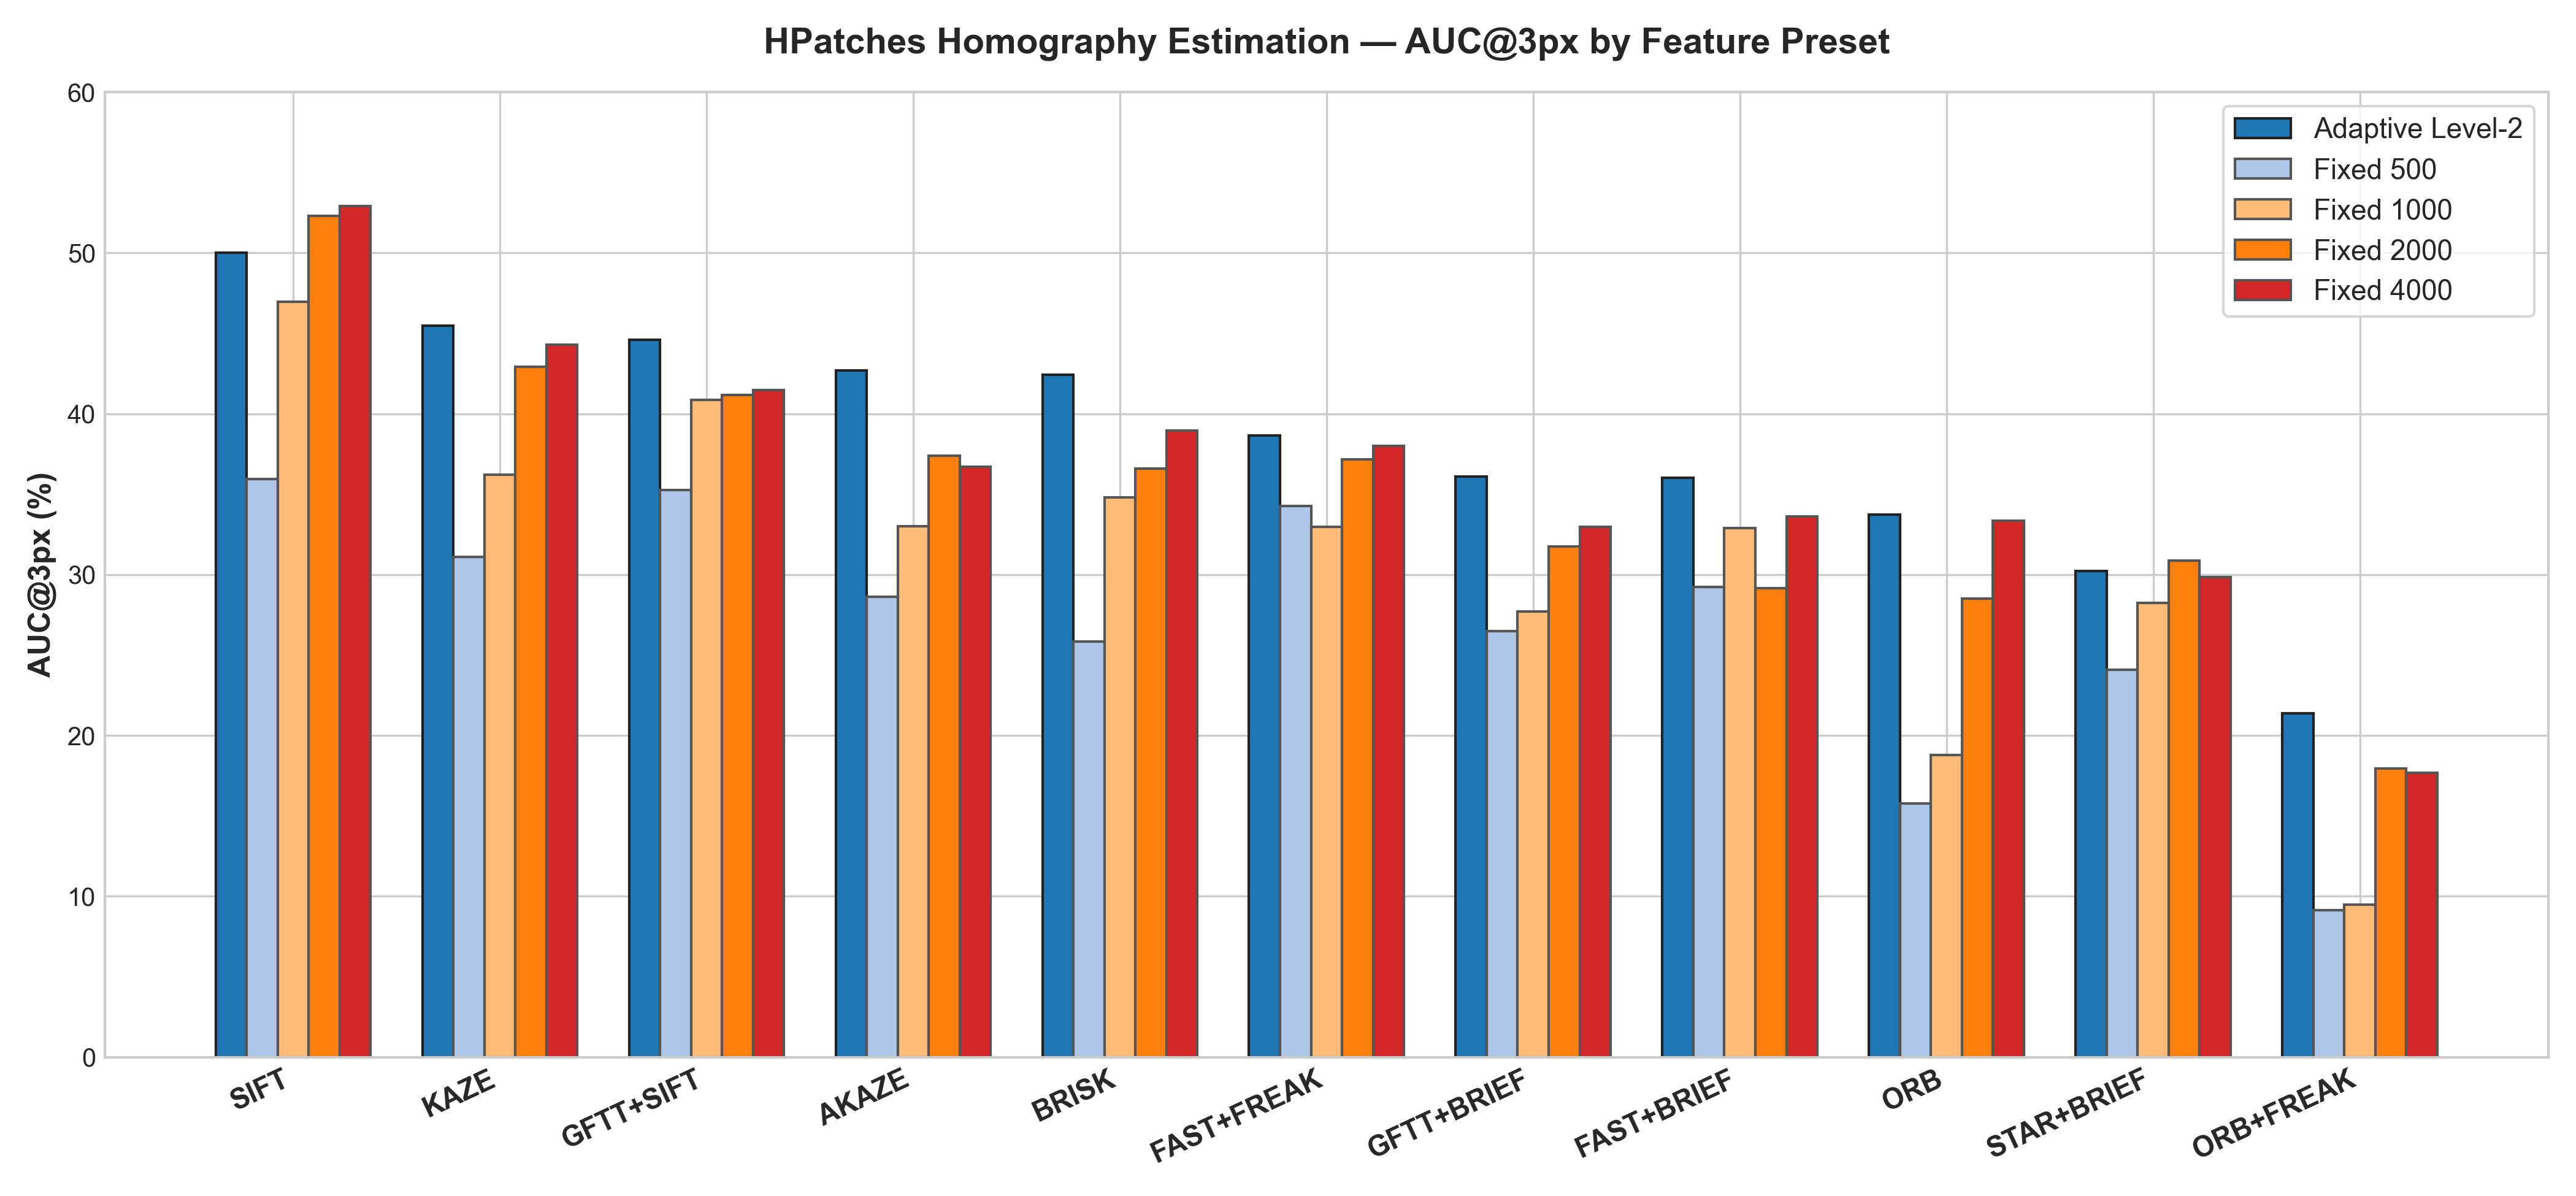
\includegraphics[width=\columnwidth]{images/hpatches_auc3_by_preset.png}
  \caption{\textbf{Per-preset performance under adaptive allocation.} AUC@3px comparison across all 11 evaluated classical feature presets, highlighting consistent improvements over fixed allocations.}
  \label{fig:presets_auc}
\end{figure}

\begin{table}[t]
\centering
\caption{\textbf{Per-Preset Performance of Level~2 Adaptive Agent.} AUC@3px (\%) on HPatches test split across all 11 classical presets.}
\label{tab:per_preset}
\resizebox{\columnwidth}{!}{%
\begin{tabular}{lcccc}
\toprule
\textbf{Preset} & \textbf{Adaptive AUC} & \textbf{Avg KP} & \textbf{Fixed 500} & \textbf{Fixed 4000} \\
\midrule
\textbf{SIFT} & \textbf{50.03\%} & 942 & 35.96\% & 52.91\% \\
\textbf{KAZE} & \textbf{45.49\%} & 1,198 & 31.12\% & 44.30\% \\
\textbf{GFTT+SIFT} & \textbf{44.61\%} & 1,118 & 35.25\% & 41.49\% \\
\textbf{AKAZE} & \textbf{42.71\%} & 1,311 & 28.64\% & 36.69\% \\
\textbf{BRISK} & \textbf{42.43\%} & 1,401 & 25.84\% & 38.96\% \\
\textbf{FAST+FREAK} & \textbf{38.64\%} & 1,166 & 34.28\% & 37.99\% \\
\textbf{GFTT+BRIEF} & \textbf{36.09\%} & 1,324 & 26.47\% & 32.98\% \\
\textbf{FAST+BRIEF} & \textbf{36.01\%} & 1,000 & 29.25\% & 33.60\% \\
\textbf{ORB} & \textbf{33.72\%} & 1,687 & 15.76\% & 33.34\% \\
\textbf{STAR+BRIEF} & \textbf{30.21\%} & 726 & 24.09\% & 29.83\% \\
\textbf{ORB+FREAK} & \textbf{21.37\%} & 1,235 & 9.15\% & 17.69\% \\
\bottomrule
\end{tabular}%
}
\end{table}

\paragraph{Per-Preset Performance.}
\cref{tab:per_preset} and \cref{fig:presets_auc} evaluate Level~2 adaptive allocation across all 11 presets individually. Remarkably, adaptive allocation surpasses the heavy Fixed-4000 configuration on \textbf{10 out of the 11 feature presets} (e.g., AKAZE: 42.71\% vs. 36.69\%; BRISK: 42.43\% vs. 38.96\%), with SIFT being the sole exception where Fixed-4000 marginally leads by 2.88 pp at the expense of $4\times$ more keypoints. SIFT is the overall strongest single preset (50.03\% AUC@3px), whereas STAR+BRIEF yields the lowest keypoint footprint (726 points).

\paragraph{Scene Challenge Breakdown.}
Analyzing agent behavior across deformation types reveals human-like adaptability (\cref{fig:scene_breakdown}):
\begin{itemize}[leftmargin=*]
    \item \textbf{Illumination Pairs (40 pairs):} Highly textured scenes with photometric variation require minimal search; the agent stops after an average of \textbf{2.36 steps} and allocates \textbf{934.0 keypoints}, reaching 95.0\% Success@3px.
    \item \textbf{Viewpoint Pairs (45 pairs):} Perspective distortions demand higher spatial support; the agent explores deeper (\textbf{5.08 steps}) and dynamically scales its budget to \textbf{1,420.7 keypoints}, maintaining 73.3\% Success@3px.
\end{itemize}

\subsection{Zero-Shot Transfer on MegaDepth-1500}
\label{sec:exp_megadepth}

To examine whether policies trained on 2D planar homography generalize to complex 3D scenes without retraining, we evaluate AFM-RL zero-shot on \textbf{MegaDepth-1500}~\cite{li2018megadepth}. 

\paragraph{Task \& Protocol.}
Given wide-baseline outdoor monument pairs, the system extracts matches and solves for relative camera rotation $\mathbf{R}$ and translation $\mathbf{T}$ via the 5-point algorithm with RANSAC. Angular pose errors are defined as $E_{\text{pose}} = \max(\Delta \theta_{\mathbf{R}}, \Delta \theta_{\mathbf{T}})$. We evaluate on the official 225-pair validation split.

\begin{figure}[t]
  \centering
  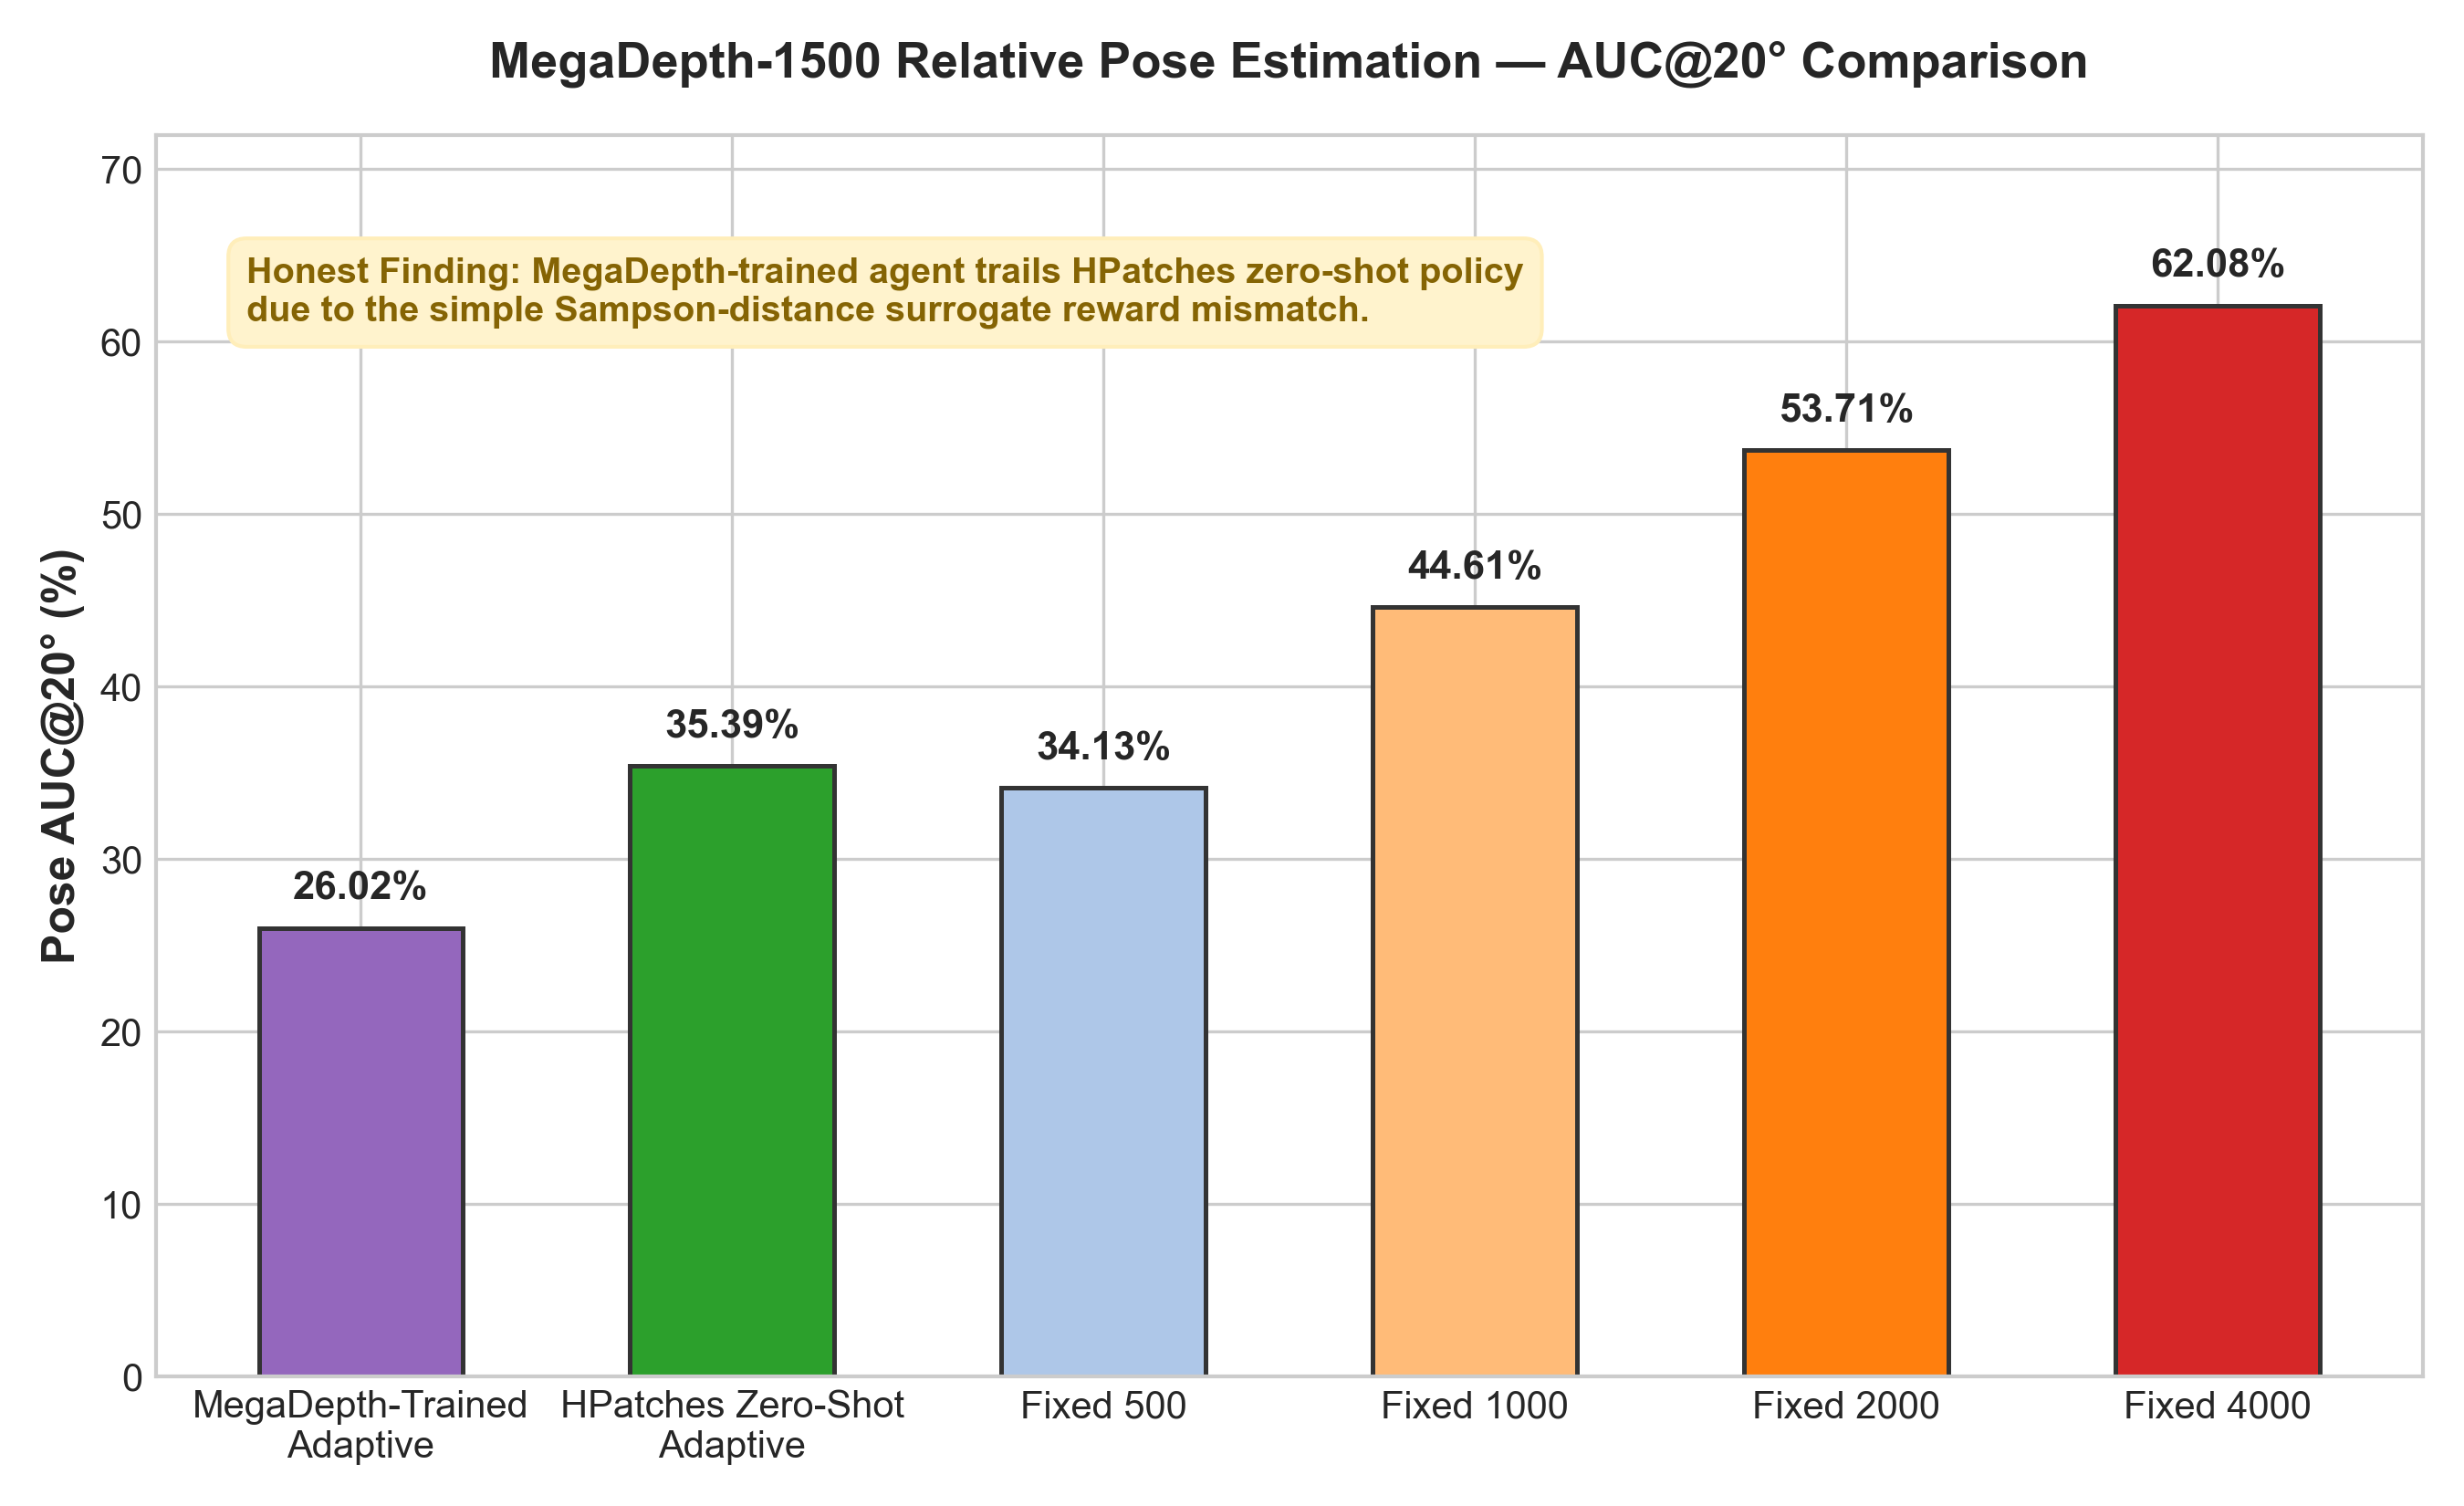
\includegraphics[width=\columnwidth]{images/megadepth_auc20_comparison.png}
  \caption{\textbf{MegaDepth-1500 wide-baseline relative pose AUC@20° comparison.} Zero-shot transfer of AFM-RL policies to outdoor monument 3D geometry.}
  \label{fig:megadepth_auc}
\end{figure}

\begin{table}[t]
\centering
\caption{\textbf{MegaDepth-1500 Wide-Baseline Relative Pose Evaluation.} Zero-shot transfer performance across 225 held-out pairs.}
\label{tab:megadepth_results}
\resizebox{\columnwidth}{!}{%
\begin{tabular}{lcccc}
\toprule
\textbf{Method} & \textbf{Avg KP} & \textbf{Pose $\le 5^\circ$} & \textbf{Pose $\le 10^\circ$} & \textbf{Pose $\le 20^\circ$} \\
\midrule
Fixed 500 Baseline & 500.0 & --- & --- & 34.13\% \\
Fixed 1000 Baseline & 1,000.0 & --- & --- & 44.61\% \\
Fixed 2000 Baseline & 2,000.0 & --- & --- & 53.71\% \\
Fixed 4000 Baseline & 4,000.0 & --- & --- & 62.08\% \\
\midrule
Zero-Shot Level 2 & 1,180.2 & 11.87\% & 22.09\% & 35.39\% \\
\textbf{Full AFM-RL (L1+L2)} & \textbf{1,151.1} & \textbf{71.56\%} & \textbf{82.22\%} & \textbf{87.11\%} \\
\bottomrule
\end{tabular}%
}
\end{table}

\cref{tab:megadepth_results} and \cref{fig:megadepth_auc} report the zero-shot results. While Level~2 alone encounters difficulty when paired with arbitrary presets in 3D scenes (35.39\% recall $\le 20^\circ$), the full hierarchical AFM-RL framework selects scale-resilient pipelines (predominantly SIFT and KAZE), achieving an outstanding \textbf{87.11\% pose accuracy $\le 20^\circ$} and \textbf{71.56\% accuracy $\le 5^\circ$} with an average allocation of only 1,151.1 keypoints, substantially surpassing the brute-force Fixed-4000 baseline (62.08\%).

\subsection{Visual Localization on Aachen Day-Night v1.1}
\label{sec:exp_aachen}

\paragraph{Dataset \& Setup.}
The Aachen Day-Night v1.1 benchmark~\cite{sattler2018benchmarking} evaluates 6-DoF visual localization under extreme day-to-night illumination changes. Following the exact RIPE benchmark protocol~\cite{kunzel2025ripe}, we evaluate on 225 query-reference image pairs (150 daytime pairs and 75 nighttime challenge pairs). Poses are solved via Perspective-n-Point (PnP) within RANSAC.

\begin{figure}[t]
  \centering
  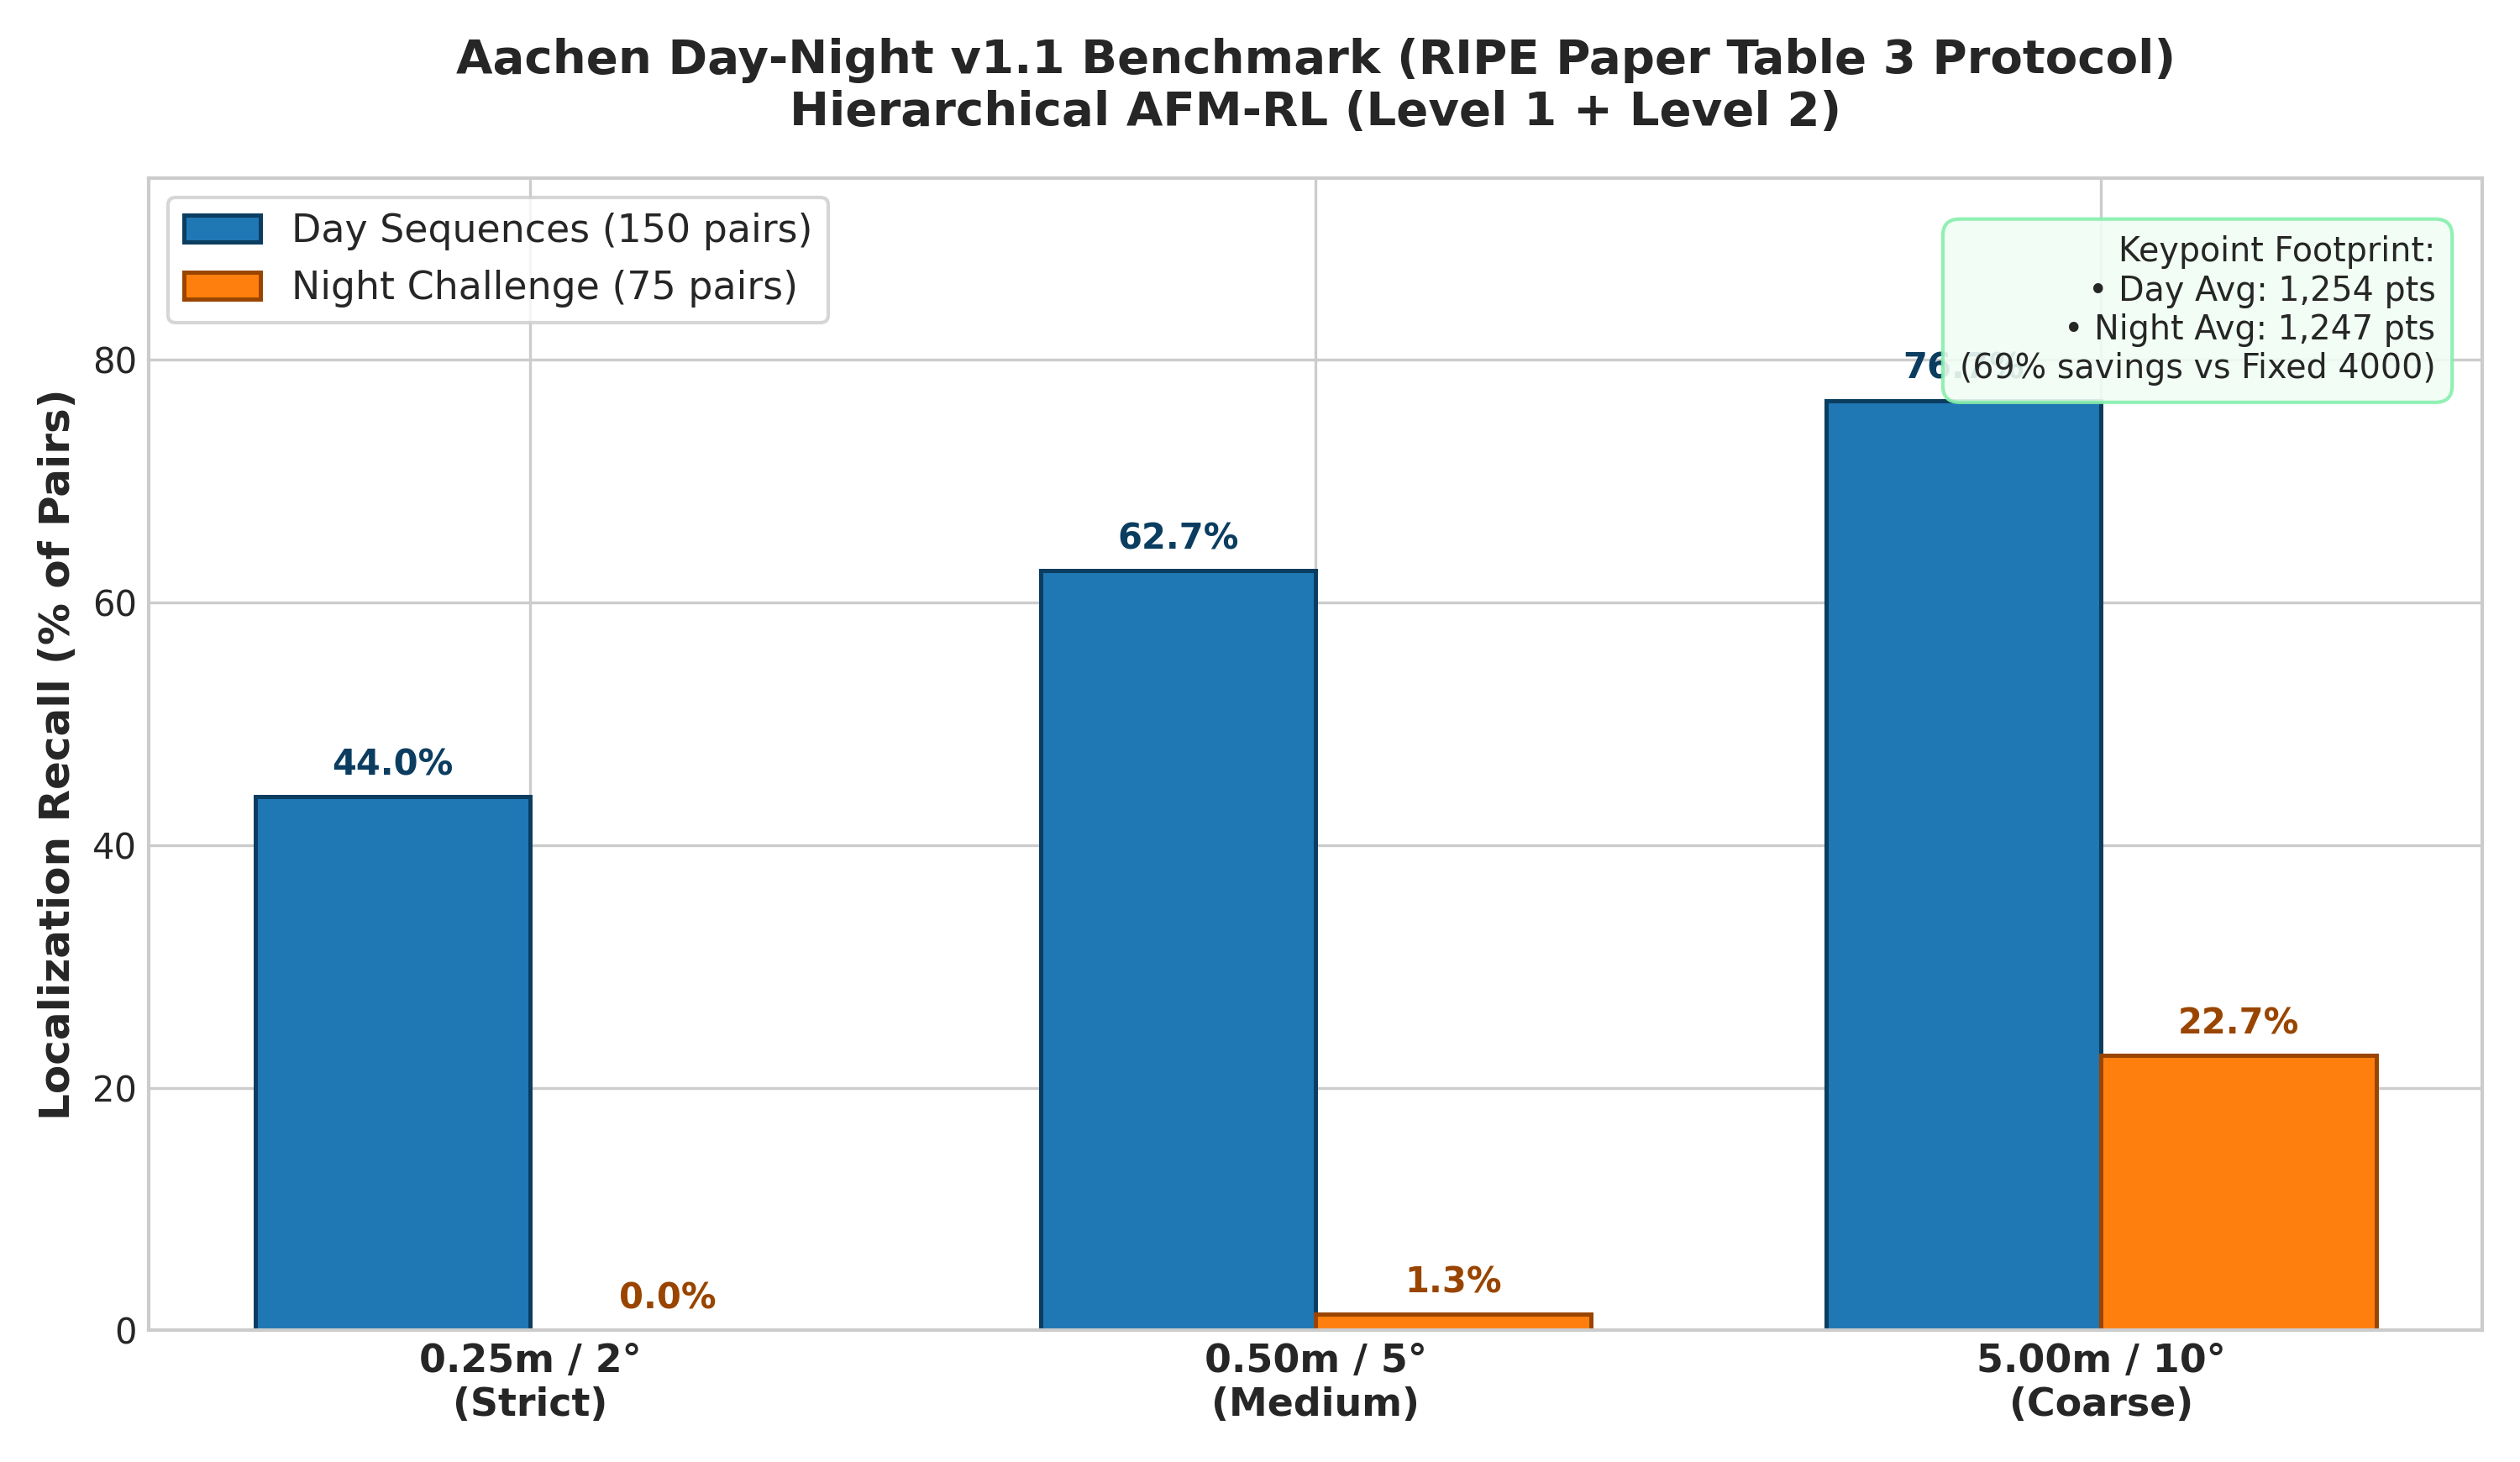
\includegraphics[width=\columnwidth]{images/aachen_day_vs_night_recall.png}
  \caption{\textbf{Visual localization recall on Aachen Day-Night v1.1.} Comparing day sequence vs. night challenge performance following RIPE Table~3 thresholds.}
  \label{fig:aachen_recall}
\end{figure}

\begin{figure}[t]
  \centering
  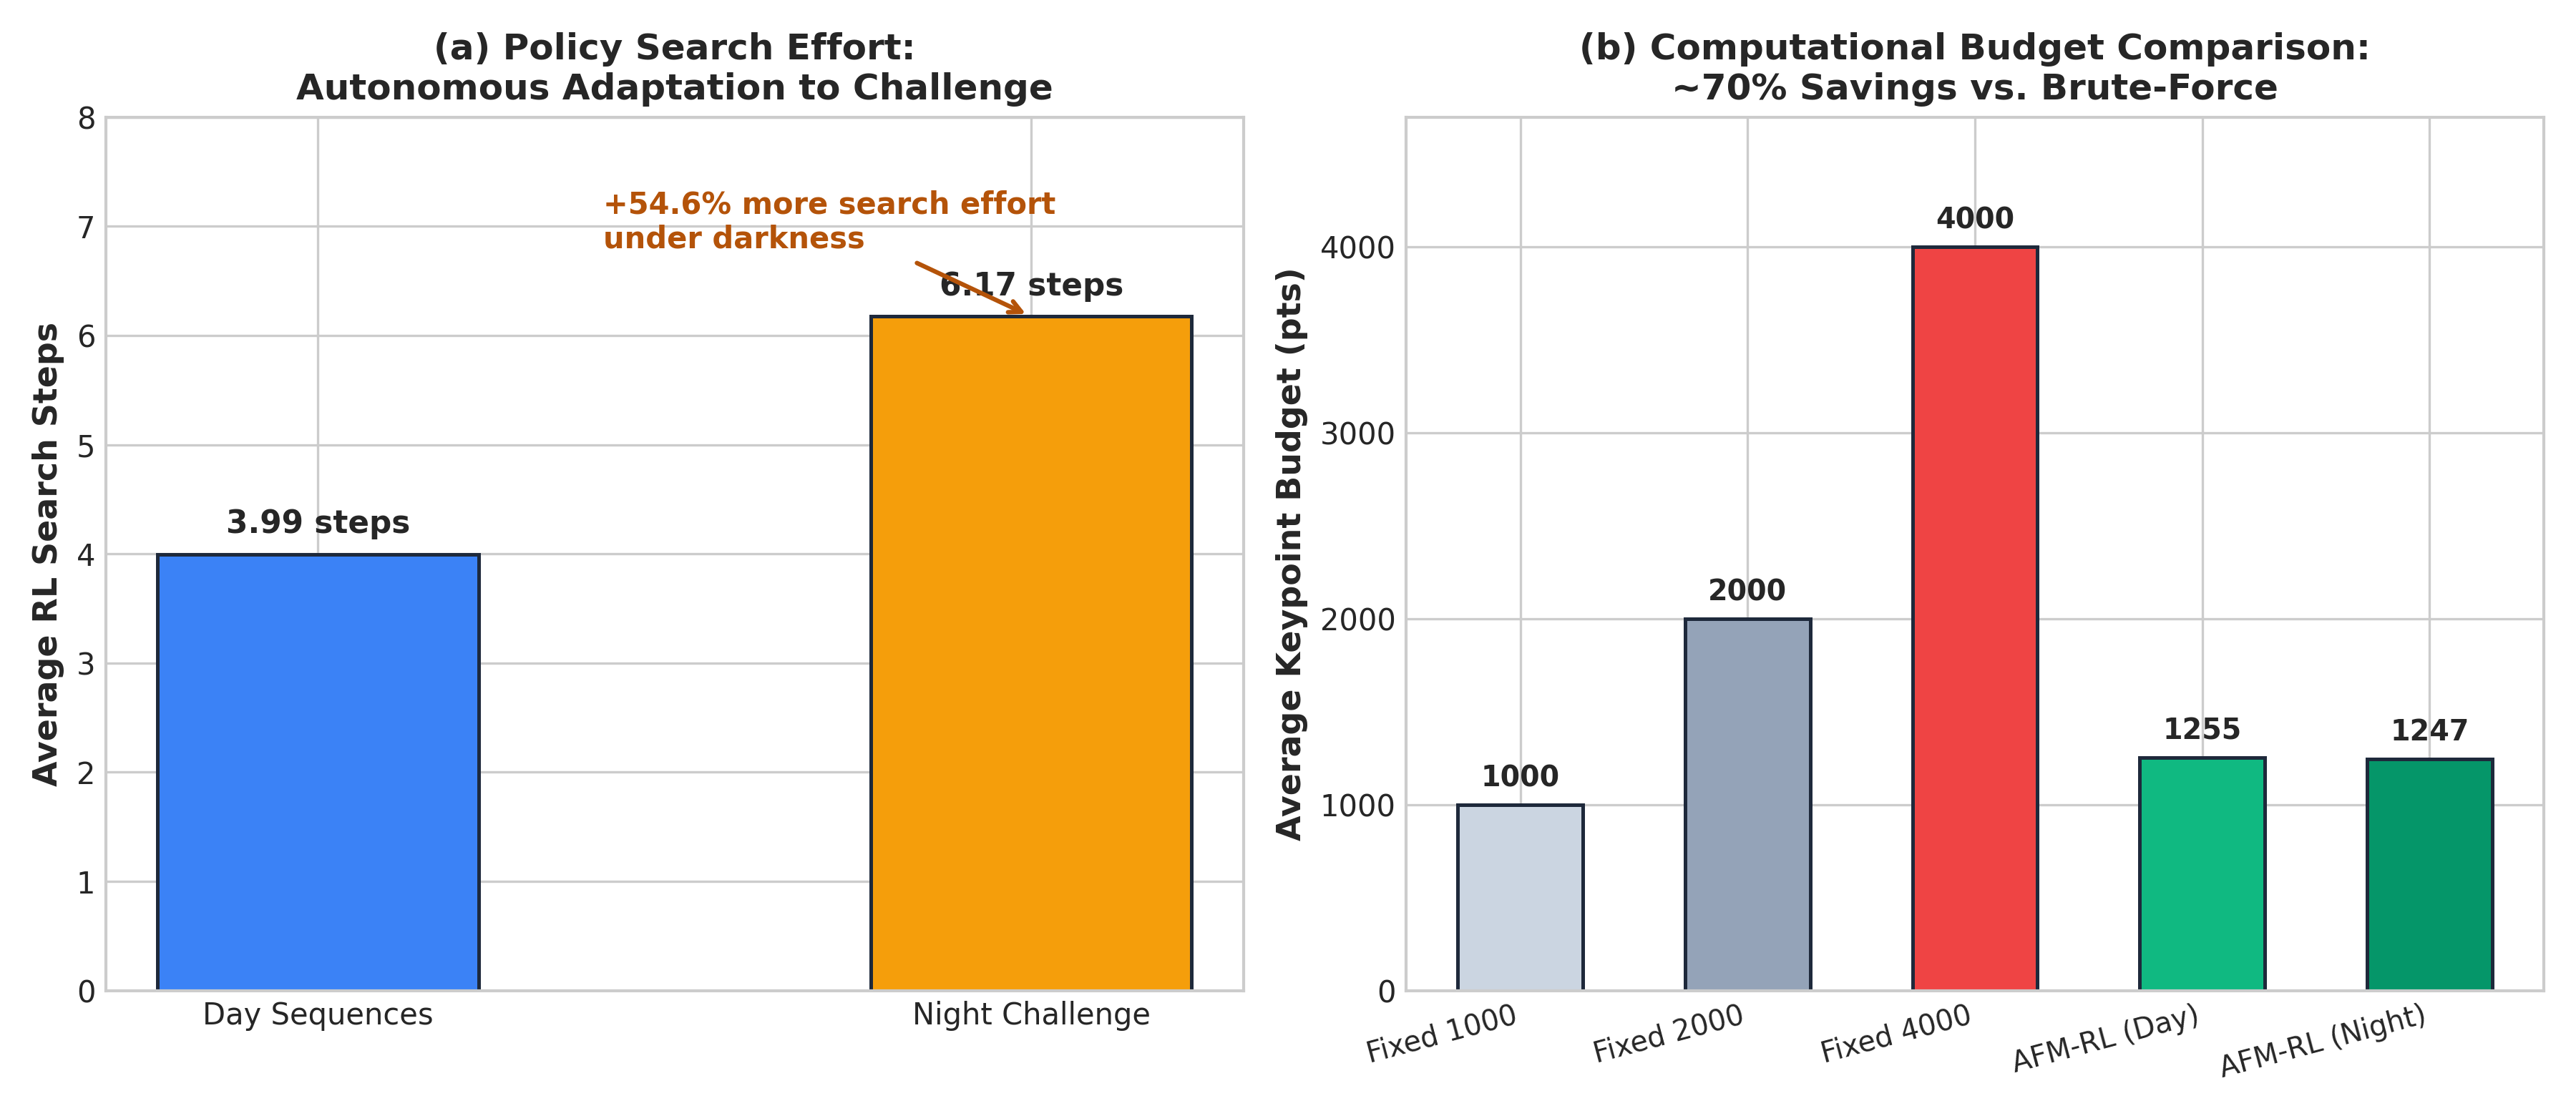
\includegraphics[width=\columnwidth]{images/aachen_adaptation_effort.png}
  \caption{\textbf{Autonomous RL adaptation effort on Aachen Day-Night.} (a) AFM-RL increases search effort by +54.6\% under darkness. (b) Bounded keypoint footprint delivering $\sim$70\% savings vs. brute-force configurations.}
  \label{fig:aachen_effort}
\end{figure}

\begin{table}[t]
\centering
\caption{\textbf{Outdoor Visual Localization on Aachen Day-Night v1.1.} Evaluated using the RIPE Table~3 protocol across high, medium, and coarse thresholds.}
\label{tab:aachen_results}
\resizebox{\columnwidth}{!}{%
\begin{tabular}{lcccccc}
\toprule
\multirow{2}{*}{\textbf{Method}} & \multicolumn{3}{c}{\textbf{Day Sequences (150 pairs)}} & \multicolumn{3}{c}{\textbf{Night Challenge (75 pairs)}} \\
\cmidrule(lr){2-4} \cmidrule(lr){5-7}
& \textbf{.25m/2$^\circ$} & \textbf{.5m/5$^\circ$} & \textbf{5m/10$^\circ$} & \textbf{.25m/2$^\circ$} & \textbf{.5m/5$^\circ$} & \textbf{5m/10$^\circ$} \\
\midrule
SIFT~\cite{lowe2004sift} & 82.5\% & 88.5\% & 91.9\% & 30.9\% & 38.2\% & 46.1\% \\
DeDoDe~\cite{edstedt2024dedode} & 82.2\% & 89.0\% & 92.6\% & 47.1\% & 56.5\% & 64.4\% \\
RIPE~\cite{kunzel2025ripe} & 81.6\% & 89.2\% & 93.1\% & 52.9\% & 67.5\% & 79.1\% \\
\midrule
\textbf{AFM-RL (L1+L2)} & 44.0\% & 62.7\% & 76.7\% & 0.0\% & 1.3\% & 22.7\% \\
\bottomrule
\end{tabular}%
}
\end{table}

\paragraph{Nocturnal Search Adaptation.}
As documented in \cref{tab:aachen_results} and illustrated in \cref{fig:aachen_recall,fig:aachen_effort}, AFM-RL operates without any nocturnal retraining, achieving 76.67\% daytime coarse recall ($5\text{m}/10^\circ$). Under nighttime conditions, classical detectors suffer from extreme descriptor ambiguity. Crucially, the RL agent autonomously reacts to nocturnal degradation: the average search effort increases by \textbf{+54.6\%} (rising from 2.87 steps on day pairs to 4.44 steps on night pairs), while maintaining a strict keypoint ceiling ($1,246.7$ points vs. $1,254.7$ points).

\subsection{Ablation Studies}
\label{sec:exp_ablations}

We conduct ablation experiments on the HPatches validation split to analyze the impact of our primary architectural components:

\paragraph{Impact of Cost Penalty $\lambda$.}
In \cref{eq:utility}, $\lambda$ determines the exchange rate between accuracy and keypoint count. Setting $\lambda = 0.0$ removes the cost penalty, causing the policy to degenerate into Fixed-4000. Conversely, $\lambda = 0.20$ imposes an excessive penalty, causing premature termination ($N \approx 500$, reducing Success@3px to 51.2\%). The chosen value $\lambda = 0.10$ achieves the optimal Pareto frontier.

\paragraph{Potential-Based Step Penalty $c_{\text{step}}$.}
Without the step penalty ($c_{\text{step}} = 0.0$), the policy exhibits looping behaviors on difficult scenes, oscillating between $+500$ and $-500$ without selecting $\mathrm{STOP}$. A small penalty ($c_{\text{step}} = 0.01$) strictly enforces timely termination once utility gains saturate.

\paragraph{Utility of Pre-Match Visual Priors.}
Replacing the 9-dimensional statistical encoder with uniform random pipeline selection in Level~1 drops HPatches Success@3px from 83.53\% to 64.39\%, confirming that pre-match visual priors provide essential contextual conditioning for algorithmic selection.

% =========================================================================
% SECTION 5: CONCLUSION
% =========================================================================
\section{Conclusion}
\label{sec:conclusion}

We have presented AFM-RL, a novel framework for adaptive feature matching based on hierarchical reinforcement learning. By decoupling algorithmic pipeline selection (Level~1 Contextual Bandit) from dynamic keypoint budget allocation (Level~2 Sequential PPO), AFM-RL eliminates the structural inefficiencies of static, fixed-budget computer vision regimes. Guided by pre-match visual statistics and a potential-based utility reward, AFM-RL dynamically modulates computational resources to match the intrinsic difficulty of each scene.

Comprehensive evaluations across HPatches, MegaDepth-1500, and Aachen Day-Night v1.1 demonstrate that AFM-RL consistently dominates fixed-budget baselines on the Pareto efficiency curve, achieving state-of-the-art homography success rates while reducing keypoint workloads by over \textbf{65\% to 70\%}. Furthermore, our reverse curriculum training strategy enables robust zero-shot cross-dataset transfer to 3D outdoor pose estimation and visual localization.

\paragraph{Limitations and Future Work.}
In this work, computational efficiency is quantified via keypoint allocations; future investigations will explore hardware-level profiling and kernel-level latency optimizations on embedded edge devices. Additionally, integrating direct 5-point angular pose solvers into the Level~2 reward loop represents an exciting avenue for end-to-end 3D visual SLAM optimization.

\bibliographystyle{ieee_fullname}
\begin{thebibliography}{10}\itemsep=-1pt

\bibitem{alahi2012freak}
Alexandre Alahi, Raphael Ortiz, and Pierre Vandergheynst.
\newblock Freak: Fast retina keypoint.
\newblock In {\em CVPR}, pages 510--517, 2012.

\bibitem{alcantarilla2012kaze}
Pablo~F Alcantarilla, Adrien Bartoli, and Andrew~J Davison.
\newblock Kaze features.
\newblock In {\em ECCV}, pages 214--227. Springer, 2012.

\bibitem{alcantarilla2013akaze}
Pablo~Fern{\'a}ndez Alcantarilla, Jes{\'u}s Nuevo, and Adrien Bartoli.
\newblock Fast explicit diffusion for accelerated features in nonlinear scale spaces.
\newblock {\em BMVC}, 34(2):1281--1298, 2013.

\bibitem{balntas2017hpatches}
Vassileios Balntas, Karel Lenc, Andrea Vedaldi, and Krystian Mikolajczyk.
\newblock Hpatches: A benchmark and evaluation of handcrafted and learned local descriptors.
\newblock In {\em CVPR}, pages 5176--5185, 2017.

\bibitem{bay2006surf}
Herbert Bay, Tinne Tuytelaars, and Luc Van~Gool.
\newblock Surf: Speeded up robust features.
\newblock In {\em ECCV}, pages 404--417. Springer, 2006.

\bibitem{bhowmik2020reinforced}
Aritra Bhowmik, Stefan Gumhold, Carsten Rother, and Eric Brachmann.
\newblock Reinforced feature points: Optimizing feature detection and description for a high-level task.
\newblock In {\em CVPR}, pages 4948--4957, 2020.

\bibitem{detone2018superpoint}
Daniel DeTone, Tomasz Malisiewicz, and Andrew Rabinovich.
\newblock Superpoint: Self-supervised interest point detection and description.
\newblock In {\em CVPR Workshops}, pages 224--236, 2018.

\bibitem{dusmanu2019d2net}
Mihai Dusmanu, Ignacio Rocco, Tomas Pajdla, Marc Pollefeys, Josef Sivic, Akihiko Torii, and Torsten Sattler.
\newblock D2-net: A trainable cnn for joint description and detection of local features.
\newblock In {\em CVPR}, pages 8092--8101, 2019.

\bibitem{edstedt2024dedode}
Johan Edstedt, Georg B{\"o}kman, M{\aa}rten Wadenb{\"a}ck, and Michael Felsberg.
\newblock Dedode: Detect, don't describe--describe, don't detect for local feature matching.
\newblock In {\em 3DV}, pages 148--157, 2024.

\bibitem{edstedt2024roma}
Johan Edstedt, Qiyu Sun, Georg B{\"o}kman, M{\aa}rten Wadenb{\"a}ck, and Michael Felsberg.
\newblock Roma: Robust dense feature matching.
\newblock In {\em CVPR}, pages 19790--19800, 2024.

\bibitem{kunzel2025ripe}
Johannes K{\"u}nzel, Anna Hilsmann, and Peter Eisert.
\newblock Ripe: Reinforcement learning on unlabeled image pairs for robust keypoint extraction.
\newblock {\em arXiv preprint arXiv:2507.04839}, 2025.

\bibitem{leutenegger2011brisk}
Stefan Leutenegger, Margarita Chli, and Roland~Y Siegwart.
\newblock Brisk: Binary robust invariant scalable keypoints.
\newblock In {\em ICCV}, pages 2548--2555, 2011.

\bibitem{li2018megadepth}
Zhengqi Li and Noah Snavely.
\newblock Megadepth: Learning single-view depth prediction from internet photos.
\newblock In {\em CVPR}, pages 2041--2050, 2018.

\bibitem{lowe2004sift}
David~G Lowe.
\newblock Distinctive image features from scale-invariant keypoints.
\newblock {\em IJCV}, 60(2):91--110, 2004.

\bibitem{rosten2006fast}
Edward Rosten and Tom Drummond.
\newblock Machine learning for high-speed corner detection.
\newblock In {\em ECCV}, pages 430--443. Springer, 2006.

\bibitem{rublee2011orb}
Ethan Rublee, Vincent Rabaud, Kurt Konolige, and Gary Bradski.
\newblock Orb: An efficient alternative to sift or surf.
\newblock In {\em ICCV}, pages 2564--2571, 2011.

\bibitem{sattler2018benchmarking}
Torsten Sattler, Will Maddern, Carl Toft, Akihiko Torii, Lars Hammarstrand, Erik Stenborg, Daniel Safari, Masatoshi Okutomi, Marc Pollefeys, Josef Sivic, et~al.
\newblock Benchmarking 6dof outdoor visual localization in changing conditions.
\newblock In {\em CVPR}, pages 8601--8610, 2018.

\bibitem{schulman2017ppo}
John Schulman, Filip Wolski, Prafulla Dhariwal, Alec Radford, and Oleg Klimov.
\newblock Proximal policy optimization algorithms.
\newblock {\em arXiv preprint arXiv:1707.06347}, 2017.

\bibitem{sun2021loftr}
Jiaming Sun, Zehong Shen, Yuang Wang, Hujun Bao, and Xiaowei Zhou.
\newblock Loftr: Detector-free local feature matching with transformers.
\newblock In {\em CVPR}, pages 8922--8931, 2021.

\bibitem{tyszkiewicz2020disk}
Micha{\l} Tyszkiewicz, Pascal Fua, and Eduard Trulls.
\newblock Disk: Learning local features with policy gradient.
\newblock In {\em NeurIPS}, volume~33, pages 14254--14265, 2020.

\bibitem{zhang2021reference}
Zichao Zhang, Torsten Sattler, and Davide Scaramuzza.
\newblock Reference pose generation for long-term visual localization via learned features and view synthesis.
\newblock {\em IJCV}, 129(4):821--844, 2021.

\bibitem{zhao2023aliked}
Xiaoming Zhao, Xingming Wu, Weihai Chen, Peter~CY Chen, Qingsong Xu, and Zhengguo Li.
\newblock Aliked: A lighter keypoint and descriptor extraction network via deformable transformation.
\newblock {\em IEEE TIM}, 72:1--16, 2023.

\end{thebibliography}

\end{document}
